\documentclass{aa}
\usepackage[varg]{txfonts}
\usepackage{color}
\usepackage{graphicx}
\usepackage{subfig}
\usepackage{bm}
\bibpunct{(}{)}{;}{a}{}{,} % to follow the A&A style
\begin{document}

\title{Real-time calibration of the AARTFAAC array for transient detection}

\author{Peeyush Prasad  \inst{1} \and Stefan J. Wijnholds  \inst{2} \and Folkert
  Huizinga  \inst{1}  \and Ralph  Wijers  \inst{1}} \institute{Universiteit  Van
  Amsterdam \and ASTRON, The Netherlands Foundation for Radio Astronomy}

\date{Received <date> / Accepted <date>}

\abstract{ The  search for transient phenomena  at low radio  frequencies is now
  coming of age with the development  of large field of view radio sky monitors,
  made  feasible by new  developments in  calibration algorithms  and computing.
  However,the accurate calibration of such arrays is challenging, especially due
  to  the  large  field of  view,  and  is  the  main  cause of  limiting  their
  sensitivities.  This paper describes  a strategy for the real-time, wide-field
  calibration  of the  Amsterdam-ASTRON Radio  Transients Facility  And Analysis
  Center (AARTFAAC) array, which  is a sensitive, continuously available all-sky
  monitor based on the Low Frequency  Array (LOFAR). The monitor will operate in
  a zenith pointing,  snapshot imaging mode for image  plane detection of bright
  radio transients.  We show that  a tracking calibration approach with solution
  propagation  satisfies   our  latency,  computing   and  calibration  accuracy
  constraints.  We characterize the  instrument and calibration strategy under a
  variety  of observing and  instrumental conditions.   These bring  out several
  phenomena  which  can bias  the  calibration.   The  real-time nature  of  the
  application further imposes strict  latency and computational constraints.  We
  find that although ionosphere induced  phase errors present a major impediment
  to  accurate calibration,  these  can be  corrected  in the  direction of  the
  brightest few  sources to significantly  improve image quality.  Our real-time
  calibration pipeline  implementation processes a single spectral  channel of a
  snapshot observation in  $\sim$ 0.2 seconds on test  hardware, well within its
  compute budget.   Autonomously calibrating  and imaging one  second snapshots,
  our approach leads  to a typical image noise  of $\sim$ 10 Jy for  a $\sim$ 90
  kHz  channel, reaching dynamic  ranges of  $\sim$ 2000:1.   We also  show that
  transient  detection sensitivity can  be significantly  improved to  reach the
  thermal limit of the array by carrying out difference imaging.}

\keywords{Radio Interferometry - Calibration - Radio Transients}

\maketitle

\section{\label{sec:Introduction}Introduction}
The detection  and characterization of low  frequency radio transients  is a Key
Science  Project \citep{fender2006lofar}  for  the Low  Frequency Array  (LOFAR)
\citep{vanhaarlem2013lofar}   radio    telescope.    In   this    context,   the
Amsterdam-ASTRON    Radio    Transients    Facility    and    Analysis    Center
(AARTFAAC) \footnote{see www.aartfaac.org }  has initiated building an All-Sky
Monitor  (ASM) to  survey most  of the  locally visible  sky for  transients and
variable sources.   The ASM  will be  an image plane  transient detector  at low
radio frequencies, with images generated  via aperture synthesis.  It will carry
out continuous, autonomous  and near real-time sky monitoring  for detecting the
brightest  ($\sim$10s  of Jy)  transients  occuring  at  a variety  of  cadences
(seconds to  minutes). Its  main aim  is rapid detection  of Low  Frequency (LF)
transients over  a large  field of  view, and the  production of  rough position
estimates  of  detected  transient  sources  for immediate  follow  up  at  high
sensitivity and resolution  with the full LOFAR array. With  its very wide field
of view, low guarenteed latency of calibration and imaging, it will enable true,
real-time  all-sky monitoring  of  the  low-frequency radio  sky  for the  first
time. Thus,  the AARTFAAC would  be the first  and most sensitive of  the coming
breed of  Radio Sky  Monitors.  Table \ref{tab:AARTFAAC_specs}  compares various
wide-field instruments with transient searches as an explicit goal.\\

The discoveries of  transients are currently biased towards  objects emitting at
higher  energies, in  the X-ray  or $\gamma$-ray  regime, primarily  due  to the
success of  various satellite  based ASMs operating  at those energy  levels. At
radio frequencies, searches  for transients have usually been  limited to mining
archives  \citep{bower2007submillijansky,bower2011search}, follow-up  studies of
discovered     transients{[}{]},    and     a     few    dedicated     observing
programs{[}{]}. However, the dynamic nature  of the sky at low radio frequencies
has not been studied in detail yet, mostly due to the restricted fields of view,
and  the low  availability of  existing instruments  for carrying  out dedicated
searches for transients.  This is set to  change with the advent of  a number of
sensitive, wide field of view (WFoV) instruments at the lowest frequencies, like
the LOFAR,  the Mileura Widefield Array  (MWA) \citep{lonsdale2009murchison} and
others.

These low-frequency instruments  should be sensitive to a  variety of phenomena,
including Pulsar giant pulses, bright  radio flares from brown dwarfs and active
stars, emission from OH masers,  Jovian bursts, and most importantly, an unknown
population of bright bursters.  Recent serendipitous discoveries of short bursts
of  bright radio  emission  of unknown  origins,  and at  low radio  frequencies
\citep{lorimer2007bright,  thornton2013population}   have  shown  the  potential
variety of  sources which  might fill  the unnaturally empty  phase space  of LF
radio transients. Thus, the development of wide field monitors like the AARTFAAC
array is timely and crucial to characterizing such sources. The science case for
the AARTFAAC is detailed in \citep{wijers2013aartfaac}.

A  variety  of  approaches  exist  for the  detection  of  transient  phenomena,
depending on factors like  the luminosity distribution, spatial distribution and
location  of  sources  (primarily  affecting  dispersion  smearing  and  scatter
broadening), their timescales  of variation, emission mechanism, as  well as the
spatial and temporal  behaviour of background noise.  These  include beam formed
observations,  deep  imaging (staring),  rapid,  shallow  imaging (tiling)  etc.
Traditionally,  image domain  transient detection  has been  considered suitable
only  for incoherent  sources of  emission, whose  timescales of  transience are
slow,  and  whose  brightness  temperatures  are  expected  to  be  <$10^{12}K$.
Coherent  sources  of  emission  have  usually been  detected  using  timeseries
analysis  of beamformed  data, although  imaging  can provide  a higher  spatial
resolution  (compared to  incoherent  beamforming)  and a  wider  field of  view
(compared to coherent beamforming), as  well as better discrimination due to the
coherent collection of power into a  single pixel.  This dichotomy is mostly due
to the  timescales of  coherent emission,  which are expected  to be  short from
light  travel time arguments,  and the  fact that  beamforming can  provide high
temporal resolutions and  sensitivities, although over a reduced  field of view.
Another  promising  alternative  for  detecting  short term  transients  is  the
bispectrum  method  of \citep{law2012all}.   This  uses interferometric  closure
quantities  from  triplets of  time  differenced  visibilities,  which makes  it
independent of  instrumental phase errors.  However,  for an array  with a large
number of elements  and low SNR per baseline,  the methods' absolute sensitivity
is lower than that  of an imaging array.  It is also  sensitive to residual flux
after the  subtraction of constant  emission from visibilities.  This  can arise
due to changes in the visibility fringe over the subtraction period, and imposes
an upper limit  on the duration of candidate transients. 

The usually sparse UV coverage in snapshot observations from imaging arrays, and
the resulting  low instantaneous sensitivities and image  dynamic ranges mandate
long  integrations for  imaging observations,  thus making  them  unsuitable for
short duration transient detection.  Another  contributor to the lack of imaging
detectors at  short timescales has been  the time consuming  step of calibration
and imaging. Recent arrays are being  constructed using a large number of small,
low senstivity elements. These provide  a perfect base for all-sky monitors, due
to their  very good instantaneous  UV coverage, high collective  sensitivity and
wide fields  of view.  The challenge of  real-time calibration and  imaging from
these  instruments  is  becoming  feasible  due to  developments  in  high-speed
calibration  algorithms as  well as  advancement in  computing  resources. Thus,
image   plane   detection  of   short   duration   bright   transients  is   now
feasible. Further, for transients with an isotropic spatial distribution,unknown
durations and luminosity  distributions, a tiling strategy of  shallow but rapid
observations would  result in  a larger number  of discovered  transients. Thus,
imaging all-sky monitors are matched for this application.

In this  paper, we  focus on  the requirements and  challenges of  the real-time
calibration component of the  transient detection pipeline.  The chosen approach
is optimized  for bounded  latency and  computing.  We begin  by laying  out the
problem  of wide-field  calibration in  the  context of  transient detection  in
Section \ref{sec:Array-calibration-for},  while describing the  approaches taken
by similar  instruments. In Section \ref{sec:The-AARTFAAC-All},  we describe the
AARTFAAC array and its suitability as a transient search machine. We then give a
detailed   description  of   our  approach   to  its   calibration   in  Section
\ref{sec:An-Optimal,-tracking},   especially  in   the  context   of  autonomous
operation. Section \ref{sec:Performance-of-tracking} presents its performance on
commissioning      data,      while      we     demonstrate      in      Section
\ref{sub:Enhancing-the-transient} that  the short-term transient  sensitivity of
the  AARTFAAC   can  be  enhanced  significantly  by   carrying  out  difference
imaging.  Section  \ref{sec:Challenges-to-tracking} elaborates  on  some of  the
challenges  faced  by  the  AARTFAAC  ASM under  real  observing  conditions, afte which we present our conclusions.

\section{\label{sec:Array-calibration-for}All-Sky calibration}
An  important requirement for  maximizing transient  detection sensitivity  is a
large field of view. However, this can make the calibration of environmental and
array  parameters  challenging.  A  wide-field  image  plane transient  detector
typically searches  image timeseries for transients by  extracting and analysing
light curves  of existing sources, or  by detecting new sources  referenced to a
database   of   lightcurves.    The   Transients   Detection   pipeline   (TraP)
\citep{swinbank2013trap}  component  of  the  AARTFAAC ASM  carries  out  source
extraction from  individual timeslices via thresholding and  fitting 2D gaussian
models to regions of emission. Hence, high point-source sensitivity and accurate
flux recovery  across the  full field  of view is  a fundamental  requirement of
calibration, while  a slight error in  source positions can be  tolerated by the
pipeline via source association.  The  flux estimation of any source via imaging
directly  depends on  the flux  calibration of  the  instantaneous visibilities,
which  in turn  depends  on a  proper division  of  the uncalibrated  flux on  a
visibility  between element  gain,  system noise  and  source flux.  Due to  the
dominance of  emission from  our own Galaxy  on system temperatures,  the system
noise can vary by almost $40\%$, depending on the pointing of the antenna. Thus,
system gain and temperature need to be continuously measured.

\subsection{\label{sub:All-Sky-cal-iono}Ionospheric effects}

The  antenna complex  gain has  contributions primarily  from the  gains  of the
electronics,  receiver  characteristics  and  telescope geometry,  but  is  also
affected at  low frequencies  by the  disturbed ionosphere, which  can act  as a
screen with temporally and spatially varying refractive and diffractive effects.
The  former affects  are  usually slowly  varying  ($\sim$hours), are  direction
independent  effects (DIEs)  and are  estimated via  observation  of calibration
sources.  The  latter, particularly  in  case  of  wide-field observations,  can
introduce a direction  dependent effect (DDE).  These can  vary on timescales of
seconds (see Section  \ref{sub:iono-effect-on-calib}), and usually require rapid
re-calibration  using the  instantaneous fluxes  and position  shifts  of bright
sources within the field.  However,  it is feasible for DDE parameter estimation
only under the  assumption that the DDE is identical for  all antennas, which in
turn is  possible only  when identical lines  of sight from  individual antennas
traverse the  ionospheric patch  with the same  refractive properties.   This is
true for compact arrays, whose  size projected to ionospheric heights is smaller
than  the typical isoplanatic  patch.  Hence,  transient monitors  are typically
wide-field compact arrays.

Calibration  of DDEs is  also necessary  to increase  the sensitivity  to weaker
transients via  adequate deconvolution of  the brightest sources to  lower their
side-lobe confusion  noise contribution to the  rest of the image  via the Point
Spread Function (PSF).  Although instrumental parameters are expected to vary on
longer  timescales (hours  to days  for LOFAR),  their precise  calibration also
mandates  temporal oversampling.  If uncorrected,  these effects  can  raise the
image noise floor  as well as contribute to variations in  the recovered flux of
sources, leading  to false positives.  Thus, real-time  calibration is necessary
for maximizing transient detection sensitivity.

An important requirement for real-time transient detection is a hard deadline on
calibration time and a limited computational budget, in view of the large number
of parameters to be estimated.  These dictate quick and timebound convergence of
the  calibration  gain  estimators.    Further,  the  streaming  nature  of  the
application and  the large number  of visibilities preclude their  buffering, as
well as multiple passes of processing. Finally, the calibration should be robust
against  sources  of  terrestrial  transients  due  to,  e.g.,  Radio  Frequency
Interference (RFI), which  can cause the algorithm to  converge to a sub-optimal
solution.

All-sky  instruments at  low frequencies  are guaranteed  to have  enough bright
sources within the  beam for in-beam calibration, and  dedicated observations of
calibrator sources  are unnecessary. Calibration  of the full FoV  (i.e., beyond
the half power  beam width) is usually necessary for  accurate estimation of the
flux contributed by  bright sources to any pointing of  the synthesized beam via
its  far sidelobes,  aiding accurate  deconvolution. 

\begin{comment}
Such an approach is not feasible for the AARTFAAC for several reasons.
Its very wide field of view results in the presence of several bright
source within a field. Further, usual aperture synthesis observations
can span long time intervals while tracking a target field, in order
to obtain the necessary UV coverage as well as the SNR on target.
Thus, a variety of direction dependent effects can limit the final
dynamic range of such synthesis images, including the effect of a
non-symmetric beam which may rotate during the course of the observation,
time variable PSF response due to changing array geometry and changing
instrumental and ionospheric contributions. This can make calibration
algorithms for such observations complex and time consuming, and thus
unideal for our requirements.
\end{comment}

Typical calibration schemes, e.g. as  implemented in the CASA package, address a
different problem than applicable to the AARTFAAC due to the restricted field of
view, much longer baselines and an  order of magnitude lesser number of stations
in typical arrays. Their algorithms  are further complicated by compensating for
higher  order  effects  like the  temporal  variation  in  the PSF  during  long
synthesis  due  to  changing   array  geometry,  rotating  non-symmetric  beams,
etc. which are moot in our application. Snapshot, zenith pointing imaging from a
co-planar array simplifies the calibration and imaging from the ASM to a certain
extent.

A  successful  approach  to  widefield  calibration  is  the  Peeling  algorithm
\citep{noordam2004peel,vdTol2007selfcallofar}, in which self-calibration towards
sources within  the field of  view is carried  out in decreasing order  of their
brightness,  with  removal  of   the  brightest  remaining  source's  calibrated
contribution  to all  visibilities. This  source is  selected via  rephasing the
array to its  direction, and the contribution of other  sources is attenuated by
averaging over their unphased  visibility contribution (fringe washing). Thus, a
single source calibration  approach is adequate, and a  Least Squares estimation
of the antenna gains in the direction of the source can be carried out using one
of  several  methods \citep{boonstra2003gain}.  The  solution  yields  a set  of
time-variable,  antenna  based  phase  corrections  per  source,  and  a  source
model.   However,  the  algorithm   requires  the   storage  of   the  estimated
visibilities,  with multiple  calibration and  imaging passes  through  the data
before  the   iterative  peeling  can   be  concluded,  and   calibrated  images
produced. This, along with the  increased computational load makes it unsuitable
for real-time operation.

Due to the compactness of the  AARTFAAC array, the additional delay along a line
of sight due to the ionosphere is  expected to be the same for all antennas. The
estimation of  a complex gain in the  direction of each source  is required, but
this can  be assumed  to be  identical for all  antennas. Thus,  a multi-source,
model  based  calibration  approach   is  appropriate  for  the  calibration  of
wide-field,  compact  arrays.    Other  contemporary  instruments  with  similar
specifications and  goals as  ours use mostly  Peeling based  approaches.  Their
specifications are compared in Table.  \ref{tab:AARTFAAC_specs}.

The MWA\citep{lonsdale2009murchison}, located in Western Australia has developed
an algorithm  for carrying out real-time, full  polarization direction dependent
calibration     of     snapshots     of     $\sim$8sec     via     a     Peeling
mechanism\citep{mitchell2008real}.   They use  the  sequential deconvolution  of
several  bright  sources in  decreasing  order of  apparent  flux,  in order  to
iteratively fit apparent angular offsets induced by ionospheric phase shifts and
antenna gains towards  these sources. This is suitable for  the much reduced FoV
of the MWA as compared to the  AARTFAAC, allowing them to fit a ``rubber sheet''
model of the  ionosphere over their FoV.  The main departure  of our approach to
theirs is in the deconvolution and the ionospheric image wander estimation.  The
sequential nature of peeling is to ensure that the sidelobe contamination of the
brighter source does  not affect the flux measurement of  the weaker source, and
hence  its deconvolution.  In  our case,  the apparent  fluxes of  the brightest
sources are  simultaneoulsy estimated, and their effects  subtracted together as
well. This is  efficient computationally, and the filled  nature of the AARTFAAC
UV plane results in low  sidelobe contamination. Further, the ionospheric effect
is estimated by fitting a phase  ramp across the available bandwidth in the MWA,
which  requires  synchronization between  the  spectrally separated  calibration
threads.   Our   estimation  uses  a   Direction  of  Arrival   (DoA)  algorithm
independently for each  spectral channel, and does not  require large bandwidths
for fitting  phase ramps.  This  allows a loosely coupled  parallel architecture
for our implementation.  The AARTFAAC  calibration has a stricter latency bound,
and  its lowered  sensitivity and  better  PSF make  an iterative  deconvolution
unattractive.

The  LWA\citep{ellingsonLWA1}   is  co-located  with  the  VLA   in  New  Mexico
(USA). Along with forming beams in real-time (its primary mode of operation), it
can  also operate  in an  'All-sky' mode  for  a single  tuning of  70 kHz.  The
calibration of antenna phases utilizes the method of Fringe rate filtering using
narrow band data to localize one of multiple point source calibrators within the
field of view. Here, the time-varying phases of visibilities due to contribution
by discrete sources is converted into a fringe rate spectrum by taking a Fourier
transform  of the  correlation,  where  the sources  are  apparent as  localized
components. The fringe  of the brightest source is  filtered, and antenna delays
extracted by  fitting a  model of  the presumed delay  response to  the measured
phase response.  Such an approach provides  a phase calibration  solution in the
unique direction of the brightest source.  However, fitting a fringe requires an
extended period of time to generate  the fit baseline, which is not suitable for
our streaming, real-time application.  Further, given the calibration approach,
the presence of a disturbed ionosphere would add a random noise on the parameter
estimates,  while any  bias due  to  ionospheric systematics  would probably  be
averaged out over the time period over which the fringe is fitted.

Field-based   calibration\citep{cottona2004beyond}  is  another   technique  for
direction dependent ionospheric phase calibration, and was developed for the VLA
74 MHz observations. Over a time  interval of 1-2 mins, it measures and converts
the apparent  position shifts of 5-10  detectable bright sources  within the FoV
into ionospheric  phase gradients over  the array. Subsequently,  an independent
phase screen (based on a 5-term basis of Zernike polynomials) is fitted onto the
observations,  and is  used  to  predict phase  gradients  in arbitrary  viewing
directions to  image the full FoV. Such  a technique is applicable  to a limited
field of view of a high sensitivity system, which implies the presence of bright
sources close enough to interpolate the phases attributed to the ionosphere. The
AARTFAAC wide  field of view  and lower sensitivitiy preclude  the interpolation
between  the widely  spaced calibrator  sources.  This implies  that sources  in
locations intermediate to model sources may be affected by ionospheric amplitude
and position variations,  which result in the presence  of structured variations
in   a   lightcurve   for   such   sources,   as   can   be   seen   in   Figure
\ref{fig:Light-curves-of}.

\section{\label{sec:The-AARTFAAC-All}The AARTFAAC All Sky Monitor System
Overview} The  AARTFAAC all-sky  monitor is an  aperture array of  288 sky-noise
limited dual  polarized dipoles (the Low  Band Antenna or LBA)  which are shared
with the LOFAR  array. These operate between 30 and 80  MHz.  They are organized
as  six stations spread  over $\sim$$350$  m, each  being a  random array  of 48
dipoles  which  can  be spatially  organized  as  one  of  a limited  number  of
configurations. The array shares its analog elements with the LOFAR array, which
thus controls  the station subarray  configuration. The received  analog signal,
after basic  analog conditioning, is baseband  sampled at 200 MHz  with a 12-bit
quantization.   All  dipoles  are  sampled  with  a  single  clock,  eliminating
differential delay  errors between antennas  due to e.g., clock  misalignment or
drift.   A hardware  digital PolyPhase  Filter Bank  splits the  $\sim$$100$ MHz
sampled band  into $\sim$$192$kHz subbands with an  8-bit complex representation
for the  subband timeseries,  which has  been found to  be adequate  to maintain
linearity  in  the  presence  of  local  RFI.  A  coupled  data  path  routes  a
configurable   subset  of   subbands   to  the   Uniboard   based  hardware   FX
correlator.  This  makes  the  AARTFAAC  a  continuously  available  instrument,
independent of ongoing LOFAR observations. No delay compensation (apart from the
fixed  cable delays)  is carried  out between  antennas, resulting  in  a zenith
poining  PSF.  The  estimation  of  the  resulting  $\sim$$1.6e5$  instantaneous
visibilities make this correlator the largest in the world in terms of processed
input  streams. I/O  restrictions  put  an input  limit  of $\sim$$66$  subbands
($\sim$$13$ MHz) to the correlator,  which produces visibilities at $24$ kHz and
one second  resolution. Note that the LOFAR  also has a High  Band Antenna (HBA)
component operating between 110 and 240  MHz, with each element being a 4x4 tile
equipped with an  analog beamformer. This implies that data  is available to the
AARTFAAC  during   HBA  observations,  which  are  mutually   exclusive  to  LBA
observations.  However, due to the limited  field of view of $\sim$$20$ deg, and
the  arbitrary pointing  of  the analog  beam of  this  system, its  use is  not
discussed further in this paper.

Table \ref{tab:AARTFAAC_specs} lists the current specifications of
the instrument. 

\begin{table*}[tbh]
\center{%
\begin{tabular}{|c|c|c|c|c|}
\hline 
Parameter & AARTFAAC LBA & MWA & LWA1 & Comment\tabularnewline
\hline 
\hline 
Array elements & 576 inverted V dipoles & 128 tiles  & 512 bowtie dipoles & \tabularnewline
\hline 
Frequency range (MHz) & 30-80  & 80-300 & 10-88 & \tabularnewline
\hline 
Field of view (sr) & $\pi$ & 0.06$\pi$  & $\pi$ & FWHM of beam\tabularnewline
\hline 
Effective area ($m^{2})$ & 10 & 21 & 2.5 & per dipole\tabularnewline
\hline 
Angular resolution (arcmin) & $\sim$$48$ & $\sim$$3$ & $\sim$$200$ & \tabularnewline
\hline 
Spectral resolution (kHz) & 24 & 40 & 75 & \tabularnewline
\hline 
Processed Bandwidth (MHz) & 13 & 30.72 & 0.075 & LWA: Narrow band Imaging\tabularnewline
\hline 
Temporal resolution (sec) & 1 & 8 & 5 & \tabularnewline
\hline 
Transient detection FoM $(Hz^{-1}S^{-1})$ & 2.3 & 1.3 & 0.830 & \tabularnewline
\hline 
\end{tabular}}

\caption{\label{tab:AARTFAAC_specs}Specifications   of   contemporary  transient
  detection instruments. The parameters are estimated at the highest sensitivity
  of each instrument, viz,  60 MHz for AARTFAAC, 150 MHz for  the MWA and 74 MHz
  for the LWA, which observes continuously only in its 'Narrow band' mode.}
\end{table*}


\subsection{\label{sub:AARTFAAC-for-Transient}AARTFAAC for Transient searches}

Temporal pulses as expected from  transients are broadened and attenuated (hence
smeared)  due  primarily  to   dispersion  and  scattering  in  the  intervening
media. The  effects are  parameterized by the  medium's dispersion  measure (DM,
$pc/cm^{-3}$),    and   are    more   enhanced    at   large    DMs    and   low
frequencies. Dispersion smearing can be  reversed via deconvolution with a known
DM,  while scatter  smearing cannot  be  reversed.  Since  pulse attenuation  is
proportional  to broadening,  transient detectors  routinely increase  the pulse
detection sensitivity by carrying out  trial DM searches.  However, the AARTFAAC
does  not carry  out de-dispersion  before  imaging.  Thus,  given the  temporal
resolution of $\sim$0.1  to 1 second of the  AARTFAAC, the transient sensitivity
achieved via  spectral collapse limits the  DM range of a  source.  The temporal
pulse broadening in seconds over a bandwidth $\Delta\nu$ MHz at $\nu$ GHz, for a
dispersion of DM units is given by Eq. \ref{eq:dm_broad}.
\begin{equation}
\Delta t_{DM}=8.3DM\Delta\nu_{MHz}\nu_{GHz}^{-3}\label{eq:dm_broad}
\end{equation}
Assuming all subbands  are chosen to be contiguous  around the peak instrumental
sensitivity while the  dispersion broadening is limited to 1  second, the 13 MHz
sensitivity  of the AARTFAAC  would be  usable for  sources with  DMs of  only a
few. Pulses from  sources at higher DMs would be broadened  beyond 1 second, and
consequently appear  at lower  SNR.  The highest  spectral resolution of  24 kHz
would allow a DM limit of $\sim$200, although at a sensitivity a factor $\sim$24
less.  An empirical relationship between  the scatter broadening time due to the
Interstellar     medium     and    the     DM     has     been    derived     by
\citep{bhat2004multifrequency}  and  implies  a  DM  limit of  $\sim$100  at  60
MHz. This upper  limit would allow larger spectral  integrations. The ability to
spread subbands over the full  analog bandwidth allows searching for ultra steep
spectrum  sources,  and  can  aid  in  distinguishing  between  terrestrial  and
celestial  transient sources.   The large  spectral baseline  will also  help in
carrying out image-based dedispersion in the future.

A   figure  of   merit  for   transient   detection\citep{cordes2004dynamic}  is
$A\Omega\left(\frac{T}{\Delta  t}\right)$,  where  A  is  the  collecting  area,
$\Omega$ is  the solid angle coverage,  T is the total  duration of observation,
and $\Delta t$  is the time resolution. Short  transient detection merits adding
an  instantaneous sensitivity parameter  for high  detection sensitivity  in the
form of the system  temperature, $T_{sys}$. Integration over bandwidth increases
sensitivity  only if de-dispersion  is carried  out.  Thus,  assuming continuous
availability and  the simultaneous imaging  of the entire  field of view,  a per
second figure of  merit is $A\Omega/T_{sys}$. Among currently  planned ASMs, the
AARTFAAC's FoM  is comparable to the LWA,  which has similar field  of view, but
would be larger considering the higher temporal and spectral resolution, and the
lower confusion noise contribution (see Table. \ref{tab:AARTFAAC_specs}).

Backer \citep{backer1999pers} has shown that  the signal to noise ratio achieved
in a  continuous widefield search  scales with the  array filling factor  $f$ as
$\sqrt{f}$. Thus, the highly sampled  aperture of the AARTFAAC dense array would
be an advantage for our application. The resulting zenith pointing PSF is stable
and repeatible in  time. At its peak sensitivity of $\sim$$58$  MHz, the PSF has
high  roll-off, low sidelobes  $\sim$$15$ dB  below peak,  with a  resolution of
$\sim$$0.8$  sq.  deg.  This implies  a  classic confusion  noise of  $\sim$$10$
Jy.  The large  number  of antennas  also  make the  AARTFAAC  a very  sensitive
instrument,     with    a     combined     $A_{eff}/T_{sys}$    of     $\sim$0.7
$m^{2}/K$\citep{wijnholds2011situ},  and  an   instantaneous  thermal  noise  of
$\sim$8 Jy,  for the standard  imaging mode of  1sec/24 kHz.  This  implies that
instantaneous images will be confusion noise, and not thermal noise limited.

The array is 2-D to high  accuracy ($\sim$1.4 cm rms in the z-axis), simplifying
wide field imaging  by eliminating the need for  W-projection or 3-D transforms.
Its compact nature implies that direction dependent antenna gains can be assumed
identical  across  antennas, enabling  their  correction  in  the image  domain.
Further, the  requirement of snapshot imaging  implies that the  sky observed by
every baseline  remains constant  within a visibility  set, thus  satisfying the
requirements of  SelfCal. Since all  dipoles are physically aligned  parallel to
each  other, the  instrumental polarization  can be  determined via  a bi-scalar
polarization calibration, and corrections can be applied in the image domain.

Dedicated  hardware is  used to  achieve low  latencies of  transient detection.
These      include     a      hardware     correlator      based      on     the
Uniboards  \footnote{http://www.radionet-eu.org/uniboard}   for  estimating  the
visibilities in  real-time, and a  software solution running on  general purpose
hardware for the calibration, imaging and transient detection pipelines.  Figure
\ref{fig:Block-diagram-depicting}  shows  the top  level  view  of the  AARTFAAC
transient  detection  streaming pipeline.   The  calibration  component of  this
pipeline is the subject of this paper.

\begin{figure*}[tbh]
\centering
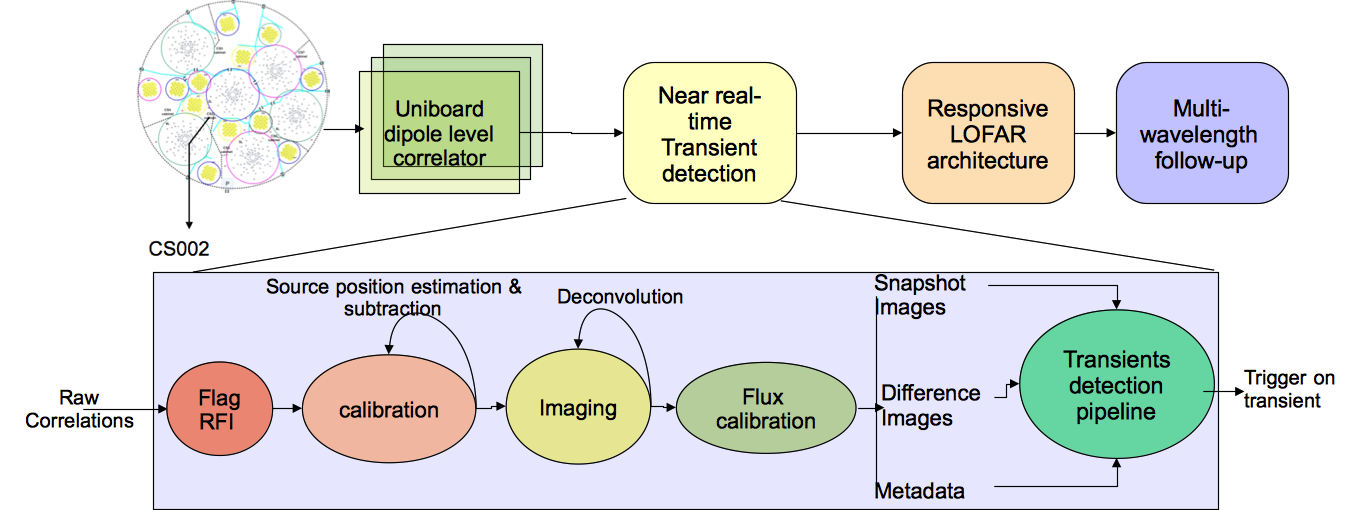
\includegraphics[width=1\textwidth]{Figs/AFAAC_blkdia_latest.png}
\caption{\label{fig:The-AARTFAAC-calibration}The    AARTFAAC   calibration   and
  imaging  pipeline within the  full ASM  flow, and  leading onto  the transient
  detection pipeline (TraP).}
\end{figure*}

\section{\label{sec:An-Optimal,-tracking}An Optimal tracking calibration
scheme for transient detection}

Here,  we present our  approach for  latency bound,  precise calibration  of the
AARTFAAC  with  a  low  computational  footprint.  We  use  a  model-sky  based,
multi-source  SelfCal approach\citep{wijnholds2009multisource}.   Calibration of
an  array  of identical,  wide-field  antennas  entails  deriving the  direction
dependent  response of every  antenna, each  of which  is excited  by multiple,
simultaneously present  calibration sources.   The system noise  contribution is
also estimated, and subtracted while  calibrating the visibilities. The input to
the  algorithm is a  running timeseries  of measured  visibilities set  from all
antennas (or the Array Correlation Matrix  (ACM)) for a given time and frequency
slice, and the corresponding instantaneous sky-model. In the following, we first
describe the calibration  of an ACM corresponding to  a single timeslice, termed
'Instantaneous  calibration'.  The  latency  and computational  constraints  for
real-time  calibration  suggest utilizing  the  available  time  axis for  rapid
convergence. This  is implemented  in the tracking  component of  our algorithm,
which  implements  a temporal  feed-forward  of  filtered  solutions as  initial
estimates.  It  may  be noted  that  our  calibration  algorithm is  limited  to
operating  in the  visibility  domain, and  does  not use  the  image domain  to
determine source structure, e.g., via CLEAN components. This is beneficial for a
streaming calibration approach.

Note that since  the telescope gains are frequency  dependent, the received band
is divided into  multiple channels, and the parameter  estimation is carried out
separately per  channel.  A  fundamental assumption is  that the  bandwidth over
which the ACM  is formed is narrow enough for phase  rotations to compensate for
temporal   delays   between  the   reception   of   the   signal  at   different
antennas\citep{zatman1998narrow}.  This  is appropriate  as the maximum  time of
flight on the longest baseline of  350 m (\textasciitilde{}1.16 $\mu s$) is much
less than the inverse of the  typical calibration channel bandwidth of $90$ kHz.
Further, tracking over the frequency axis  is not utilized due to the ability of
the  AARTFAAC to  sparsely place  frequency  bands in  order to  fully span  the
available band.


\subsection{Instantaneous calibration}

Array  calibration  can  be  formulated  as a  non-linear  parameter  estimation
problem,  which  can  be   resolved  using  statistically  efficient  estimators
generated via a Non-linear Least Squares approach. Our approach to calibrating a
single      incoming      timeslice       closely      follows      that      of
\citep{wijnholds2009multisource},  which  establishes  asymptotically  efficient
estimators   for   the   model   parameters  via   a   Maximum-Likelihood   (ML)
formulation. Given a set of $p$ antennas whose locations are known precisely and
$q$ calibration sources  within the field of view, the  data model developed for
the instantaneous ACM $R$ in their scheme is given by:
\begin{equation}
\mathbf{R=GAG_{0}\Sigma_{s}G_{0}^{H}A^{H}G^{H}+\Sigma_{n}}\label{eq:datamodel}
\end{equation}
where    \textbf{$\mathbf{G=}diag(\left[g_{1},\ldots,g_{p}\right])$    }is   the
diagonal matrix of DIE gain of each antenna, $\mathbf{A}$ is the matrix of array
steering vectors,  generated using  the known positions  of the  array antennas,
$\mathbf{G_{0}=}diag(\left[g_{01},\ldots,g_{0q}\right])$ is  the diagonal matrix
of    DDE   gain    in   the    direction    of   each    model   source    $q$,
$\mathbf{\Sigma_{s}}=diag\left(\left[\sigma_{s1}^{2},\ldots,\sigma_{sq}^{2}\right]\right)$
is the  known flux  of the  sources in the  sky model,  and $\Sigma_{n}$  is the
diagonal  noise covariance  matrix assuming  an uncorrelated,  but non-identical
system noise contribution from each antenna .

The model parameters to solve for are of the form:
\begin{equation}
\bm{\theta}=[\gamma_{1},\ldots\gamma_{p},\phi_{2}...,\phi_{p,}\sigma_{s1}^{2},...\sigma_{sq}^{2},\mathbf{l_{1}}^{T},...\mathbf{l_{q}}^{T},\sigma_{n1},...,\sigma_{np}],\label{eq:estparam}
\end{equation}
 where $\mathbf{\gamma_{i}}$  is the direction independent gain  of each antenna
 and $\phi_{i}$ is the  associated phase. $\sigma_{si}$ and $\mathbf{l}^{T}$ are
 the estimated fluxes and positions of the model sources, while $\sigma_{ni}$ is
 the system noise, assumed to be independent for each antenna.

Since  all  signals  are  assumed  to be  independent,  identically  distributed
Gaussian random variables, the Normal  Equations for this estimation problem are
generated by minimizing the negative log-likelihood function:
\begin{equation}
\bm{\hat{\theta}}=argmin\left(ln|\mathbf{R(\theta)}|+tr(\mathbf{R}^{-1}(\theta)\mathbf{\widehat{R}})\right)\label{eq:normeq}
\end{equation}
 where $\mathbf{R}(\theta)$ is the model  covariance matrix as a function of the
 parameters  $\theta$,  and  $\mathbf{\widehat{R}}$  is  the  sample  covariance
 matrix.

Due to  the difficulty in  solving this minimization  problem in closed  form, a
numerical  optimization based on  a weighted  least squares  covariance matching
estimation technique (COMET)  is utilized \citep{ottersten1998covariance}.  This
is known to  lead to estimates that  are equivalent to ML estimates  for a large
number  of  samples,  thus  being  asymptotically  efficient  and  reaching  the
theoretical  limit of the  error on  the estimator,  the Cramer-Rao  lower bound
(CRLB).

The estimation  of the  instantaneous calibration parameters  is carried  out by
partitioning  the parameters into  subsets, and  then alternating  between least
squares solutions of individual subsets. This approach of using the best current
estimate of a subset in an iteration to estimate the other subsets of parameters
is called Weighted Alternating Least Squares (WALS).


\subsubsection{\label{sub:Model-generation}Model generation}

Forming the  normal equations of  Eq. \ref{eq:normeq} for  minimization requires
modeling    the    observed   visibilities    using    the    data   model    in
Eq. \ref{eq:datamodel} and the current  estimates of the parameters.  Due to the
limited resolution of  the array, most of the brightest  objects (apart from the
Galactic plane) are unresolved by the AARTFAAC.  Thus, the sky can be modeled by
a collection of points  at the nominal location of the bright  sources. We use a
sky model composed of the brightest  sources in the sky, viz., CasA, CygA, VirA,
TauA and the point Sun, whose  nominal positions are determined from the revised
Third cambridge catalog (3CR). The model parameters used are summarized in Table
\ref{tab:Details-of-model}. The efficacy of  this model for parameter estimation
is      elaborated      upon      using      real      data      in      Section
\ref{sub:Direction-independent-gain}.   Of these model  soures, CasA  is visible
throughout the year from the location of the AARTFAAC. Galactic emission, having
a steep spectrum, is extremely bright at LOFAR frequencies and also difficult to
model due to the detailed  structure resolvable at the AARTFAAC's resolution and
sensitivity. Hence, we  filter out the low spatial  frequencies to suppress this
emission during calibration. The model can  then account for a large fraction of
the received flux on the filtered visibilities, and is constrained by the fluxes
and  positions of  the model  sources, as  well as  the noise  model.  The model
building   requires    an   estimate   of   the    actual   instantaneous   flux
$\left(\mathbf{\Sigma_{s}}\right)$ of the model  sources, along with the current
estimate of the  direction independent gain solutions and  the noise. Typically,
an  accurate Selfcal  sky  model provides  the  model fluxes  as well.  However,
significant  flux  variation of  the  model sources  can  be  introduced by  the
ionosphere  over  the AARTFAAC  array  as well  as  by  the direction  dependent
gain.  Hence, estimating  the model  source  fluxes via  an efficient  estimator
results   in    the   generation   of   a   consistent    sky   model.   Section
\ref{sub:Direction-dependent-gain}  summarizes   this  approach.  Note   that  a
relative flux stability  is more relevant for a  transient detection instrument,
and can  be achieved to  a higher accuracy  than an absolute flux  extraction. A
COMET based estimator for the noise  covariance has been shown to be well suited
if a  linearly parameterized model  of the noise  covariance matrix is  used for
this  problem\citep{ottersten1998covariance}.  However,  antennas in  a  crowded
array  like the  AARTFAAC  can mutually  couple  with each  other, resulting  in
coloring  of the  noise. Our  noise  model also  includes such  effects, and  is
discussed in more detail in Section \ref{sub:System-noise-estimation}.
\begin{comment}
 Values  of  A-team   and  galactic  plane  contribution  is   based  on  actual
 contribution to visibilities in night time data (for CasA/CygA and Galaxy), and
 day  time data  for  VirA,TauA and  the  Sun.  The  total  power of  calibrated
 visibilties = sum(abs(acccalgal(:)).^2), where acccalgal = (gainsol' * gainsol)
 .* acc; The Galactic contribution  = sum (abs(sigman(:)).^2), but also includes
 the autocorrs, which is  a sum of Tsys and Tsky, and  which cannot be separated
 without external measurements of Tsys. This explains the high value of galactic
 contribution, against an expected 40% contribution.  The RAteam contribution is
 estimated by generating model  visibilities from fluxes estimated by LSimaging,
 ie, the apparent  flux, and so is elevation dependent.  NOTE  that we dont have
 observations in which  all Ateam sources are at high  elevations, in which case
 we multiply their visibility contribution by the approximate beam attenuation.
    SNR was removed from the table, as it does not provide very much extra information as compared to the total flux contribution from a source.
\end{comment}
\begin{table*}[tbh]
\center{%
\begin{tabular}{|c|c|c|c|c|}
\hline 
Src & $S_{60}(Jy)$ & 74 MHz Size  & \% total flux  & Comment\tabularnewline
\hline 
\hline 
3C461 (CasA) & 19605.31 & 7' & $\sim$0.04 & Baars spectra, helmboldt decay\tabularnewline
\hline 
3C405 (CygA) & 19201.65 & 4.5' & $\sim$0.04 & Baars spectra\tabularnewline
\hline 
3C144 (TauA) & 2417.31 & 8' &  & Baars spectra\tabularnewline
\hline 
3C274 (VirA) & 1656.46 & 14' & $\sim$0.006& Helmboldt spectra\tabularnewline
\hline 
Sun (quiet) &  &  & $\sim$0.06 & \tabularnewline
\hline 
Galatic plane &  &  & $\sim$85.5 & Rogers spectra\tabularnewline
\hline 
\end{tabular}}
\caption{\label{tab:Details-of-model}Details of  model sources used  for All-sky
 Selfcal.   The $S_{60}$  has  been  generated using  the  spectral indices  of
 \citep{helmboldt2008radio}, while  a secular decrease  in the flux of  CasA of
  -0.8\% has been assumed. }
\end{table*}

\subsubsection{Selfcal constraints in tracking calibration}

Since the  gain estimator does  not have a  closed form solution,  the iterative
algorithm for gain estimation needs  to be appropriately constrained in order to
guide  the  optimization towards  the  global  minima  and a  physically  viable
solution in every iteration.\\

Typically, constraints  on the estimated  parameters based on the  positivity of
source emission, confinement of source structure, conservation of the total flux
of model sources etc. are used.  However, the variability of model source fluxes
due to  ionospheric scintillation prevents using  the conservation of  flux as a
constraint  in our context.  Doing so  couples the  estimated gain  solutions to
variability  in  the  model  fluxes,  thus  transferring  the  scintillation  to
calibrated visibilities, and  hence over the entire field of  view.  In order to
break  this  coupling, we  instead  utilize a  constraint  on  the average  gain
amplitude over all antennas, setting it to unity. This reflects the behaviour of
antenna  gain amplitudes,  which were  observed to  be stable  to a  few percent
across all antennas and over  long times during commissioning observations.  The
phases  are referenced  to  the first  antenna  in the  array  as an  additional
constraint.  These  constraints guide  the  traversal  of  the $\chi^{2}$  error
surface towards an identifiable  global minimum, whose convergence is identified
by a slow enough rate of change of the estimated parameters.


\subsubsection{\label{sub:Direction-independent-gain}Direction independent gain
estimation (Minor Cycle)}

Once  an appropriate  model  for  the observed  visibilities  has been  created,
direction independent gains can be estimated using an appropriate estimator. The
AARTFAAC   calibration    is   latency    bound,   hence   we    implement   the
StEFCal\citep{salvini2013stef}  algorithm for  gain estimation.   This algorithm
scales   as   $\mathcal{O}(N^{2})$   for    N   parameters,   as   against   the
$\mathcal{O}(N^{3})$  scaling  of traditional  solvers,  thus  providing a  huge
speed-up of the  calibration process.  This is primarily  due to linearizing the
cost  function, allowing  the solution  to  be computed  analytically and  hence
avoiding the  need for  matrix inversions which  are essential in  other solvers
like  the Levenberg-Marquardt  minimizer. This  algorithm has  been shown  to be
unbiased, and  with good convergence.  The StEFCal implementation  increases the
throughput  of calibration  by  a  factor $\sim$30  in  our application,  making
real-time calibration of every time and frequency slice feasible.


\subsubsection{\label{sub:Direction-dependent-gain}Direction dependent gain estimation
(Major Cycle)}

\textbf{\emph{Model   source  flux   estimation:}}  As   explained   in  Section
\ref{sub:Model-generation}, instantaneous  estimates of the  total (deconvolved)
model source  flux are required for model  generation.  This can be  framed as a
parameter estimation  problem, for  which a closed  form estimator based  on the
COMET  approach has  been  developed in  \citep{wijnholds2008fundamental} in  an
approach called Least Squares Imaging.  Here, the array configuration is assumed
known to a high accuracy, while  the number of sources requiring flux estimation
is assumed to be smaller than the  number of resolution elements in the field of
view.  This  approach allows  the  deconvolved  flux of  a  model  source to  be
estimated, due to  the incorporation of a deconvolution operator  as part of the
estimator. Figure  \ref{fig:Estimated-flux-of} shows  the extracted flux  of the
brightest visible  model sources,  and clearly shows  the effect of  the element
beam and ionospheric scintillation.

\textbf{\emph{Bias  of the  flux  estimator:}}\emph{ }An  interesting aspect  of
estimating with a COMET approach was  seen in the SelfCal bias due to unmodelled
flux leading to  an over-estimation of the model source  fluxes during the least
squares  imaging  step.  This was  attributed  to  the  fact that  although  the
calibrated  visibilities have  only a  minimal contribution  from  the spatially
filtered  visibilities, the  applied  covariance matched  weighting (whose  best
estimate  is  the   observed  ACM)  did  have  contributions   from  these  same
visibilities.  This mismatch  caused the  flux estimation  of the  model sources
being  overestimated by  an  amount  corresponding to  the  contribution of  the
unmodeled sources in  the filtered visibilities. As a result,  we have seen that
these  baselines should  also  be removed  from  the weighting  matrix prior  to
carrying out the estimation of the model fluxes. This prevents overestimation of
the  source  flux,  which has  implications  both  on  calibration, as  well  as
deconvolution. Thus,  the flux estimation is  carried out using  only the longer
baselines, which results  in the SelfCal bias now  being mitigated to acceptably
low levels. \textcolor{red}{<Too much detail?  Pedestrian language?>}

\textbf{\emph{Model   source    position   estimation:}}\emph{   }The   tracking
calibration approach  also incorporates a  Direction of Arrival  (DoA) algorithm
using   a   vector  subspace   technique   called   Weighted  Subspace   Fitting
(WSF)\citep{viberg1991detection}. This  allows us to  estimate the instantaneous
direction  of a  model source,  thus compensating  for the  image wander  of the
sources due to  ionospheric refraction. The WSF is  an algorithm for determining
the directions  of multiple  narrow-band, far-field emitters  whose uncorrelated
signals are  received by an arbitrary (but  known) array geometry. It  is a high
resolution algorithm, with a  resolution $<\frac{\lambda}{D}$ (D being the array
size) possible  for sources  with a  high SNR. It  operates by  partitioning the
received ACM  into a signal and  a noise subspace based  on its eigen-structure.
It then confines the signal subspace corresponding to the true signal parameters
to  the subspace  spanned by  the array  manifold vectors,  which  represent the
functional dependence of  the array response vector to a  source over the region
of interest  in parameter  space. Then, the  signal parameters are  estimated by
finding the best least-squares fit of the two subspaces. A crucial assumption is
that the  array manifold  is known,  implying that the  array is  calibrated. To
satisfy this  requirement, our approach generates  initial calibration solutions
based on  the catalog positions of  the model sources, calibrates  the array and
then carries out a WSF estimation. Further, the WSF initial DoA estimates can be
the catalog  positions of the model  sources. An example of  estimation with the
WSF  on test observations,  and its  spatial resolution  is presented  in Figure
\ref{fig:Deviation-of-the}.\\   \textbf{\emph{Bias  of   the   WSF  estimator:}}
\textcolor{black}{The  requirement for the  majority of  flux in  the ACM  to be
  contributed by the  model sources imply that the  algorithm can produce biased
  solutions in the  presence of unmodeled flux. Tests of  the WSF show {[}insert
    memo (tbd){]} that spatial filtering  of the diffuse emission is adequate to
  prevent this biasing.}

Thus,  WSF along with  LS imaging  allows us  to accommodate  the effect  of the
ionosphere into  the model visibilities,  leading to lower modeling  errors, and
hence better estimates of the calibration parameters.  Calibrating the data then
requires applying  the DIE solutions  to the incoming  data, while the  DDEs are
corrected in the image plane via a beam model which incorporates the effects.

The instantaneous calibration of a  single time-frequency slice of AARTFAAC data
can hence be  split into a Major  cycle of DIE, DDE and  noise estimation, while
within each Major cycle, multiple Minor cycles of DIE estimation are carried out
using the latest estimates of the other parameters. This is depicted pictorially
in Figure \ref{fig:Block-diagram-depicting}.

\begin{figure*}[tbh]
\centering
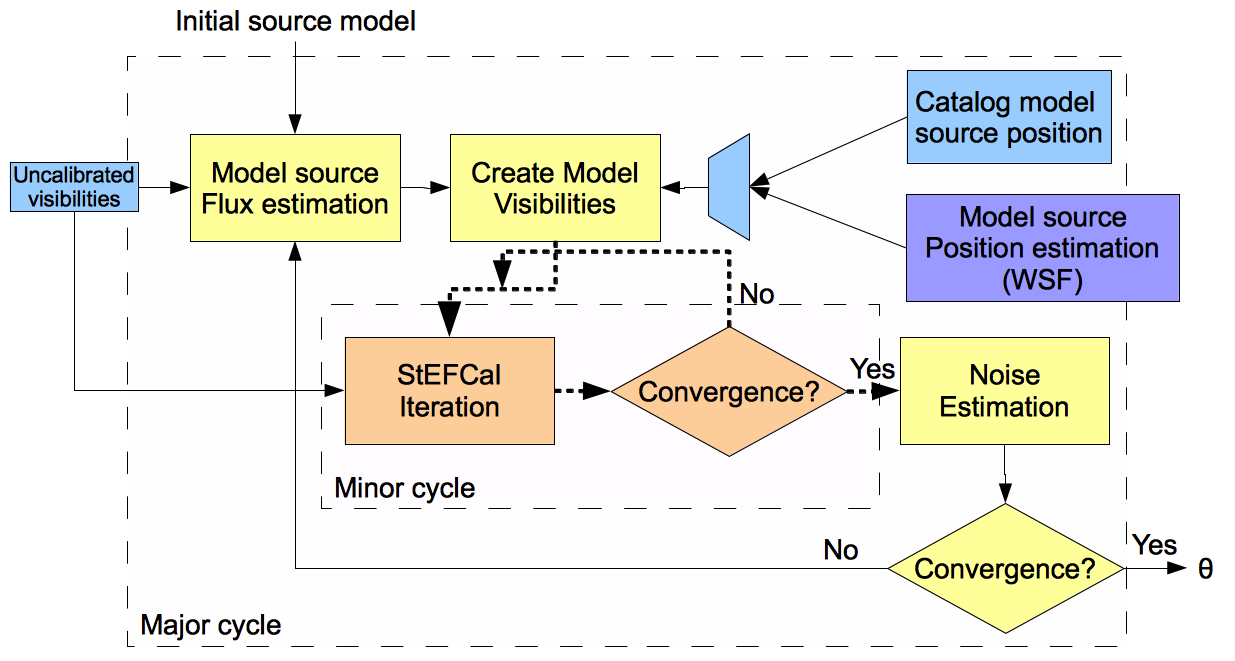
\includegraphics[width=0.8\textwidth]{Figs/Fig2_blkdiag}\caption{\label{fig:Block-diagram-depicting}Block diagram depicting the snapshot
iterative calibration control flow in the AARTFAAC optimal calibration
scheme. }
\end{figure*}

\subsubsection{\label{sub:System-noise-estimation}System noise estimation in the
presence of Galactic emission and antenna mutual coupling}

Both Galactic  emission and coupling  between closely spaced antennas  can cause
correlation  noise on  the visibility  formed from  a pair  of  antennas. Mutual
coupling due to  the antennas being placed closer than half  a wavelength at the
lower frequencies can result in fluctuation  of the PSF gain and sidelobe levels
as a function of pointing direction\citep{agrawal1972mutual}.  This implies that
antenna  pattern multiplication  (assuming that  a  single element  of an  array
behaves similarly  to it  being isolated)  may not apply.  Mutual coupling  is a
short baseline effect, and can be  ignored between the antennas of the different
stations making  up the AARTFAAC. The  impact of mutual coupling  to the antenna
primary beam  in the typical  LBA\_OUTER mode of  observation is expected  to be
$<-17dB$ from simulations\citep{wijnholds2011situ}.

The very bright synchrotron background  of the Galactic plane at low frequencies
also poses problems. Firstly, the total system noise temperature being dominated
by Galactic emission  also leads to correlated noise  between antennas. This, in
turn, again  leads to poorer  sensitivity of the  PSF formed by  including these
baselines as a function of pointing  direction and away from the zenith compared
to   the   sensitivity  expected   after   pattern   multiplication,  as   found
by\citep{ellingson2011sensitivity}.   They also  found  that the  effect of  the
Galactic  correlated noise  dominates  that due  to  mutual coupling,  and is  a
function of  the location of  the Galactic plane  within the field of  view. The
Galactic noise correlation  is expected to reduce significantly  after a few 10s
of wavelengths separation  between antennas forming a baseline,  and so can also
be termed a short baseline effect.

Secondly, the Galactic plane presents a hard to model source due to its extended
nature  (10s  of  degrees  around  the  Galactic  equator).   Even  if  modeled,
calibration can be  complicated by a model with far  larger number of parameters
than a point source model. Finally, for high sensitivity transient detection its
contribution to the  image brightness needs to be subtracted  due to the limited
dynamic range of the generated images.

The  coupling  effects   and  the  correlation  of  Galactic   noise  have  been
phenomenologically   modeled  in   \citep{wijnholds2010self}   by  an   additive
non-diagonal  noise covariance  matrix  (defined  over a  limited  set of  short
baselines) in the measurement equation. A weighted alternating least squares (or
WALS) approach  is taken  to estimate the  parameters in the  non-diagonal noise
covariance  matrix. This  allows a  simple  point source  model to  be used  for
calibration,   leading    to   a    lower   bias   in    calibration   parameter
estimates. Further,  the calibrated  visibilities can subtract  the contribution
due  to  mutual  coupling,  correlated  sky  noise,  as  well  as  the  receiver
temperatures of  each antenna  and achieve a  PSF with higher  sensitivity. This
approach,   however,    leads   to   the   situation    described   in   Section
\ref{sub:Direction-dependent-gain} of a  biased flux estimator, whose resolution
is also  described in the  same section.  Hence,  all our estimators  ignore the
short baselines (defined  as $<10\lambda$) to avoid the  interaction between the
excess flux at the shortest baselines and the calibration parameters.

%% In practice, it has been seen that the estimated values of the non-diagonal
%% covariance matrix are a substantial fraction of the total received
%% flux on the selected short baselines. Thus, the calibrated visibilities
%% have an inherent taper or 'hole' in the visibility plane which can
%% lead to ringing in the image domain, and needs to be tapered. 

%% The oversampled UV plane of the AARTFAAC allows implementing a spatial
%% filter with high roll-off and low sidelobes (put numbers?). In practice,
%% a filter with a $10-20\lambda$ cutoff has been found to be effective.
%% The filter taper is implemented in the form of a surface of revolution
%% of a gaussian to reduce ringing in the image domain.

\subsubsection{Bandpass calibration}

The ASM  operates in  a narrow-band  mode by default.  The incoming  raw complex
voltages from each antenna are organized as several subbands of $\sim$$192$ kHz,
which  are further  filtered to  give  the correlator  u2spectral resolution  of
$\sim$$30$  kHz. These  subbands can  be spread  anywhere within  the  $100$ MHz
baseband bandwidth via  the configurable hardware, and as  such sample different
components  of  the  receiver  bandpass.  The ASM  generates  channel  collapsed
calibrated  visibilities for  imaging spanning  multiple subbands  and typically
over a MHz. However, the LBA bandpass  can have variations of upto 80\% from the
peak  resonance   at  $\sim$$58$  MHz\citep{vanhaarlem2013lofar}.Thus,  bandpass
calibration  is necessary,  and the  calibrated visibilities  are scaled  by the
known bandpass response of the  LBA unilaterally. This is adequate to spectrally
collapse  narrow  bandwidths, and  allow  a  multi-frequency  synthesis mode  of
imaging.


\subsubsection{Flux density calibration}

The low resolution of the AARTFAAC allows  the use of a number of bright sources
for    calibrating     visibility    amplitudes.     Recently,     Scaife    and
Heald\citep{scaife2012broad} have  modeled the low frequency  spectra of several
bright  and   compact  sources  to  provide  a   low-frequency,  broadband  flux
scale. Their set  of six sources span the  full RA range, while due  to the very
wide field of view of the AARTFAAC, a few of these sources are typically visible
in  every snapshot.   Hence, the  AARTFAAC fluxes  are tied  to this  scale. The
dipole  primary beam  response is  derived from  a  full-polarization simulation
incorporating all  antennas of the  AARTFAAC with individual ground  planes. The
simulation incorporates the effects  of mutual coupling between closeby antennas
{[}Arts, beamsim{]}. An  average response over all antennas is  then used as the
primary beam  response, which is  applied as a  correction to the full  field of
view in the image domain.

Table \ref{tab:Flux-ratios-of-1} presents the  ratio of the integrated fluxes of
several  bright  sources  in  test  observations  to  the  expected  value  from
literature.  The integrated  fluxes are  generated  by fitting  2D Gaussians  to
sources  detected in  a snapshot  image,  and taking  the volume  of the  fitted
Gaussian. Light curves  are then generated for the  various observations. A mean
integrated flux in  pixel counts is estimated by first  segmenting the data into
100 sec. blocks, finding  the median of each block, and then  taking the mean of
the medians.  The  calibrated fluxes of several bright  sources within the field
of view  are then compared with  those derived from literature,  as indicated in
the comment column.  The dominant source of  error to the flux ratios  is due to
ionospheric scintillation,  which creates structured noise at  timescales of 10s
of seconds. Another  contributor is the error in modeling  the primary beam. The
fluxes from VLSS  have been scaled to  60 MHz assuming a spectral  index of 0.7,
while the $S_{60}$  for CasA and CygA has  been taken using the VLA  74 MHz flux
from \citep{kassim200774},  with a spectral  index (and the  frequency dependent
secular  flux decrease)  published  by Baars  et. al.  \citep{baars1977absolute}
spectral index  fits. The deviations from  published fluxes are  acceptable to a
transient detection system as long as systematics are absent. This is seen to be
true due to the limited range of fit errors on the calibrated sources.

\begin{table*}[tbh]
\center{%
\begin{tabular}{|c|c|c|c|c|c|c|c|}
\hline 
Source & $S_{60}$ (Jy) & $\sigma_{S_{60}}$ & Calibrated & error & Ratio & Cnt/Jy & Comment\tabularnewline
 &  &  & flux (Jy) & (Jy) &  &  & (vals derived from dataset 3\tabularnewline
\hline 
3C10 & 367.9 &  & 397.02 & 0 & 1.08 &  & VLSS 4 comp.\tabularnewline
\hline 
3C452 & 152.2 &  & 184.52 &  & 1.21 &  & VLSS 2 comp.\tabularnewline
\hline 
3C390.3 & 99 &  & 121.89 &  & 1.23 &  & VLSS 3 comp.\tabularnewline
\hline 
3C380 & 156.2 &  & 156.2 &  & 1 &  & Scaife et. al\tabularnewline
\hline 
3C295 & 134.5 &  & 95.23 &  & 0.71 &  & Scaife et. al\tabularnewline
\hline 
3C405 & 19202 &  & 26927 & 78 & 1.402 &  & Kassim et. al.\tabularnewline
\hline 
3C461 & 16145 &  & 31758 & 89 & 1.967 &  & Kassim et. al.\tabularnewline
\hline 
\end{tabular}}\caption{\label{tab:Flux-ratios-of-1}Flux ratios of bright sources within
a snapshot. The $S_{60}$ flux has been derived from modeled spectra.
The calibrated flux ratio is derived after imaging the calibrated
visibilities.}
\end{table*}



\subsection{Tracking calibration}

%% The main requirements for calibrating the AARTFAAC array can now be
%% summarized as:
%% \begin{itemize}
%% \item A large number of calibration parameters to estimate (antenna elements
%% + dir. Dependent params), hence computationally expensive (large matrix
%% operations).
%% \item Requirement of bounded latency for real-time operation. 
%% \item Need for rapid calibration to closely track variations in instrumental
%% and environmental parameters.
%% \end{itemize}
An  Alternating   Least  squares  approach   is  already  known  to   have  high
computational  efficiency   over  closed  form  estimators,  as   well  as  fast
convergence  \citep{boonstra2003gain}.   Thus   this  approach  is  particularly
suitable for  our case due to  our latency and compute  budgets.  However, Least
squares  algorithms  are quite  sensitive  to  an  initial estimate,  which  can
otherwise lead to convergence to local minima. Due to the high temporal sampling
of the calibration parameters, a very good initial estimate can be the solutions
from  a  previous timeslice.   Thus,  considering  the  known stability  of  the
instrument   (see  Sec.    \ref{sub:Stability}),  and   the   required  frequent
re-estimation of the calibration  parameters, we optimize the computational load
of the  algorithm by reducing the  number of iterations of  the iterative solver
per timeslice  to just one. This  is supplemented by  propagating solutions from
previous timeslices as  initial estimates for the model  parameters, which keeps
the  algorithm  on track.  Spectral  stability can  also  be  utilized to  track
solutions in the frequency axis, however, we  choose to use the time axis due to
the possibility  of the  AARTFAAC subbands being  chosen to sparsely  sample the
full  bandwidth in  order to  optimize detection  of steep  spectrum transients.
Note  that computationally,  Stefcal  iterations are  relatively inexpensive  as
compared to e.g.,  WSF (see Table. \ref{tab:Performance-results}. This implies that  their number can be
increased  in order  to handle  data with  higher errors  with little  effect on
latency bounds.  Thus, the results from  a single iteration show  the worst case
calibration (and best case computational) performance of our approach.

The feedback of solutions as initial estimates makes our approach susceptible to
errors in case  of bad data leading to incorrect solutions.   We prevent this by
maintaining a  short time window of  solutions, against which  all new estimates
are compared  before being  used for feedback.   In case  of a bad  solution, an
average gain  over the window  is used.  This  approach works well  to eliminate
biases in estimates due to incorrect tracking.

\emph{StEFCal  and tracking: }The  StEFCal algorithm  already utilizes  the gain
estimate  from a  previous  iteration. Although  it  is seen  to converge  quite
rapidly even for  a very poor estimate, initialization with a  gain close to the
truth  leads  to even  more  rapid  convergence.  This  can  be  seen in  Figure
\ref{fig:Convergence-behaviour-of}, which compares  the number of iterations and
the residuals for an identical timeslice, with no initial gain estimate, and one
determined from the previous timeslice.

Finally, several heuristics have been put in place for handling exceptional data
cases which can derail the tracking  calibration due to the constant feedback of
incongruous  calibration solutions  to future  initial estimates.   The tracking
calibration algorithm can be summarized as follows:
\begin{enumerate}
\item Carry  out a  calibration to convergence  over the  first time slice  in a
  chosen temporal window at a specified spectral resolution. This determines the
  baseline of parameter estimates.
\item For every time and spectral bin within a window:
\item Estimate positions of model sources via DOA estimation techniques.
\item Carry  out a  single iteration of  all minimization procedures  within the
  algorithm,  using  the previously  generated  baseline  parameters as  initial
  estimates.
\item Compare updated parameter  estimates for temporal and spectral smoothness.
  If  deviant solutions  found, reject  as bad  solutions, return  previous good
  solution.
\end{enumerate}
A  computational profile  of  the  various algorithmic  components  of both  the
convergent  and   the  tracking  calibration   schemes  is  depicted   in  Table
\ref{tab:Performance-results}. A  schematic view of  the tracking calibration  and its
major          components          is          shown          in          Figure
\textcolor{black}{\ref{fig:trackcalSchematic}.}

\begin{figure}[tbh]
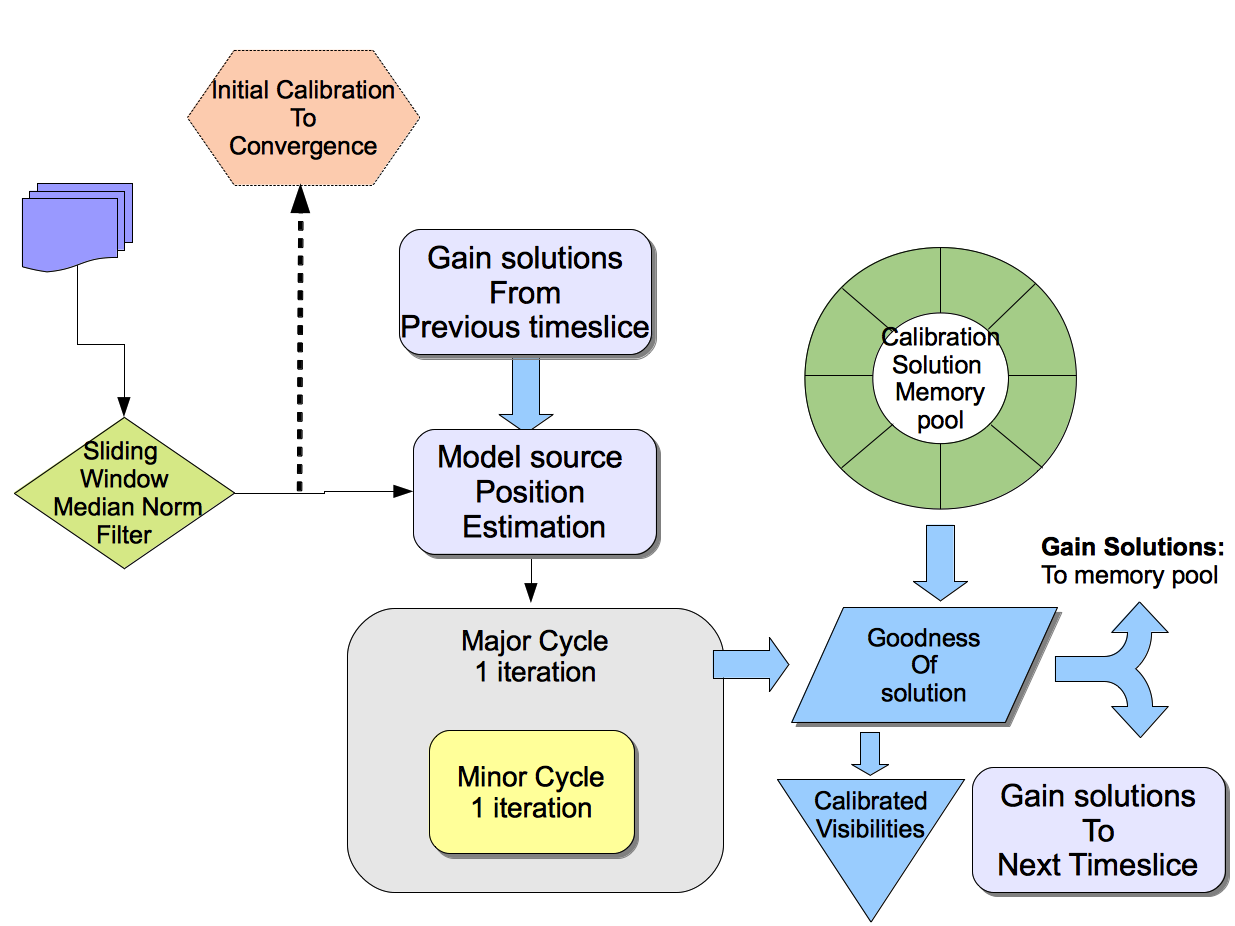
\includegraphics[width=1\columnwidth]{Figs/tracking_cal_schematic}

\caption{\label{fig:trackcalSchematic}Schematic view of tracking calibration
for bounded latency precise calibration.}
\end{figure}

\section{\label{sec:Performance-of-tracking}Performance of tracking calibration}

In this section, we present  some results of using tracking calibration obtained
on commissioning  data. Due  to the hardware  per-dipole correlator  still being
under development,  these data were obtained  via a unique mode  of operation of
the LOFAR. Here, the beamformer weights of all antennas in a station were set to
0, except  for one antenna,  whose weight was  set to 1. Passing  the sub-banded
datastream  through the  beamformer then  resulted  in a  single dipoles's  data
appearing as a beamformed output,  these were subsequently recorded to disk. The
LOFAR  hardware allows  the  continuous recording  of  5 subbands  from all  288
dual-polarized  AARTFAAC   antennas  in  this  mode.   These  were  subsequently
correlated offline before further processing and analysis.

In this section,  we examine some of the different  observing conditions that an
autonomous calibration algorithm will encounter, and evaluate its performance in
those conditions.  Our metric of  performance is two-tiered: We  first establish
the calibration efficiency of our approach  on a single time and frequency slice
by comparison  against theoretically expected  thresholds. During this  test, we
set high  convergence thresholds in order  to extract the  best performance from
the  calibration  parameter  estimators.  We  refer to  this  estimator  as  the
'convergent calibration' estimator.

We next compare the calibration  efficiency of the tracking approach against the
previously established best  performance. Here, we carry out  a single iteration
of both  the Major and Minor  cycles, providing the minimum  latency and compute
requirements.\\  \emph{Data Description:  }Data corresponding  to  the subbanded
timeseries  from  each antenna  of  the  AARTFAAC  array were  recorded  between
1200-1500  UTC,  21Sep2011, and  again  throughout  the  night of  12Jul13.  The
stations were in  the LBA\_OUTER array configuration during  all observations to
facilitate comparisons. The salient details of the observations are tabulated in
Table. \ref{tab:Details-of-commissioning}.

\begin{table*}[tbh]
\center{%
\begin{tabular}{|c|c|c|c|c|c|c|}
\hline 
Sl.no & Duration & $\Delta t$ & $\Delta\nu$ & Nchan & $\nu_{obs}$ & Comment\tabularnewline
\hline 
\hline 
1. & 21Sep2011: 1200-1500 UTC & 5s & 3 kHz & 64{*}5 & 60 MHz & Active Sun \tabularnewline
\hline 
2. & 12Jul2012: 2222-2258 UTC & 1s & 3 kHz & 64{*}5 & 60 MHz & Slow scintillation\tabularnewline
\hline 
3. & 12Jul2012:0140-0200 UTC & 1s & 3 kHz & 64{*}5 & 60 MHz & Rapid scintillation\tabularnewline
\hline 
4. & 12Jul2012:0500-0600 UTC & 1s & 3 kHz & 64{*}5 & 60 MHz & Local dawn\tabularnewline
\hline 
\end{tabular}}

\caption{\label{tab:Details-of-commissioning}Details of commissioning observations
carried out with the AARTFAAC }
\end{table*}



\subsection{Calibration accuracy on a single timeslice}

In this section, we elaborate on the convergence behaviour of the calibration on
a typical data  segment, while commenting on the aspects  of weighting for model
source flux estimation  and Selfcal constraints.  A timeslice  from Dataset 3 is
used for this analysis, and could be considered typical in terms of data quality
and  observing  conditions.   This  data  is however,  affected  by  significant
scintillation, which  is expected  for wide field  instruments. The  fraction of
data    affected    by    RFI     in    the    Low    Band    is    surprisingly
small\citep{offringa2012lofar},   and   is   not   considered  to   affect   our
conclusions. Figure \ref{fig:Convergence-behaviour-of}  shows the typical number
of major and minor cycle  iterations taken for convergence via their convergence
curves. We see  that for a default  initial estimate of antenna gains  of 1, the
DIE  calibration  converges in  10s  of  iterations,  with a  steep  convergence
curve. This is a motivation to apply tracking calibration for the AARTFAAC.

%% \begin{figure*}[tbh]
%% \subfloat[Typical minor cycle convergence of StefCal in the first major cycle.
%% Note the steep slope initially.]{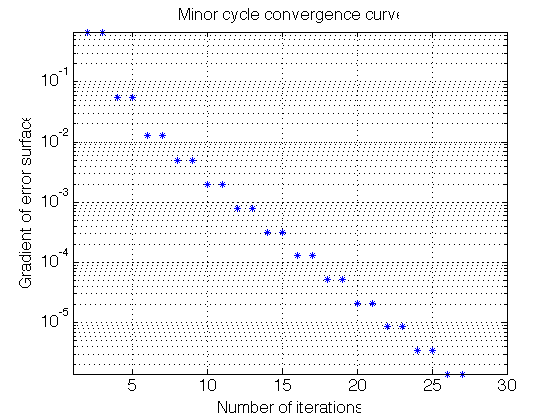
\includegraphics[width=1\columnwidth]{Figs/stefcal_convergence_1st_calext}

%% }\subfloat[Major cycle convergence.]{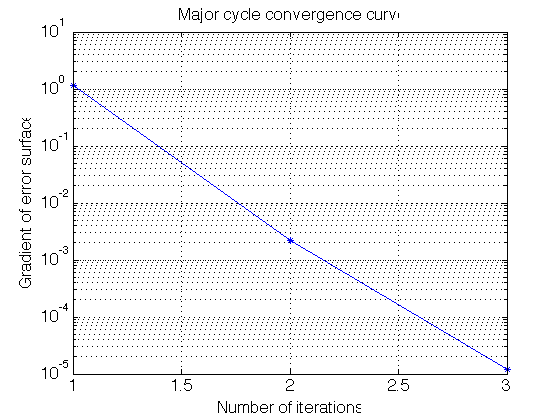
\includegraphics[width=1\columnwidth]{Figs/calext_convergence}

%% }

%% \caption{\label{fig:Convergence-behaviour-of}Convergence behaviour of Major
%% and Minor cycles of an instantaneous calibration.}
%% \end{figure*}

\begin{figure}[tbh]
%% \centering
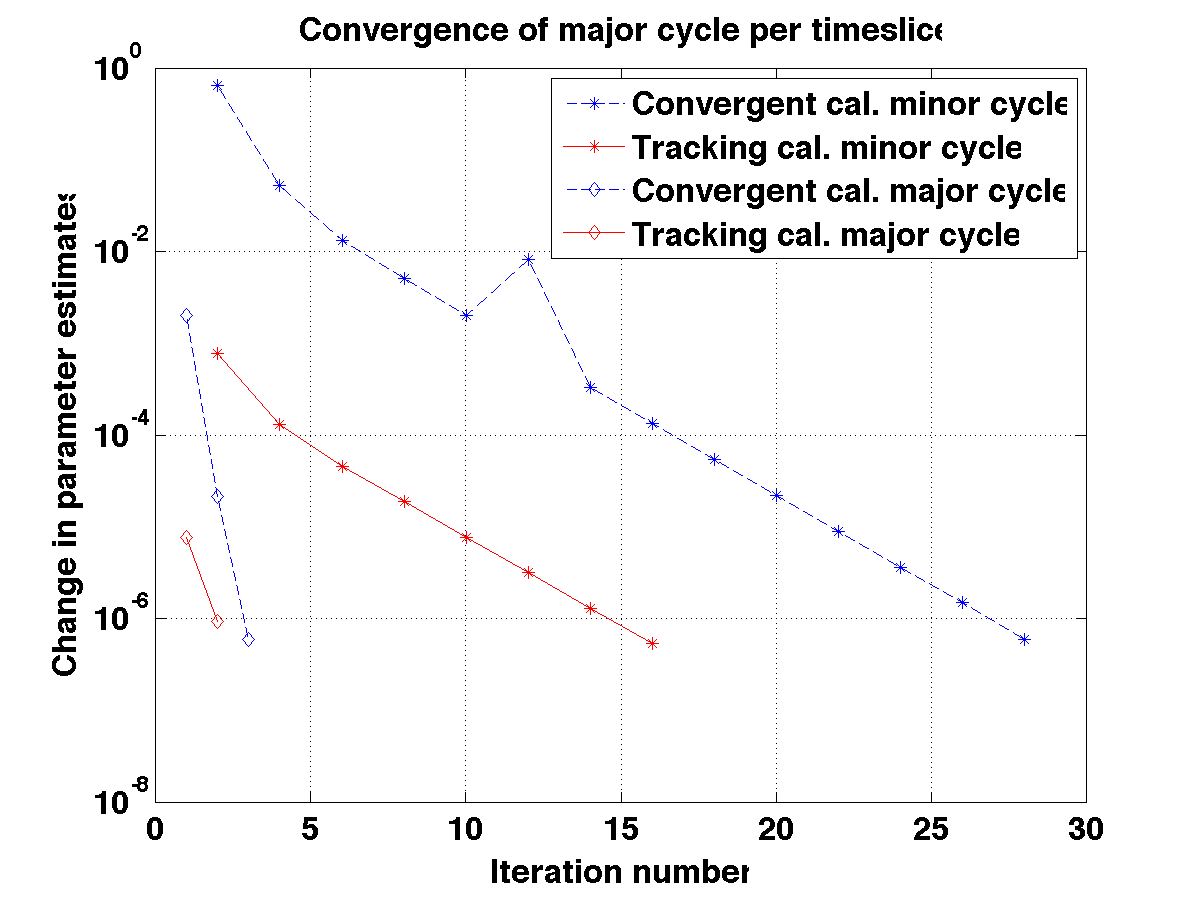
\includegraphics[width=1\columnwidth]{Figs/major_minor_cycle_conv.png}

\caption{\label{fig:Convergence-behaviour-of}Typical   major  and   minor  cycle
  convergence rates on  a single timeslice. The stars  indicate calibration with
  no prior knowledge of gain solutions, as used in convergent calibration, while
  the diamonds  show the convergence rate after  pre-initializing with solutions
  from a previous timeslice.}
\end{figure}

\textbf{\emph{Model efficacy:  }}The parameters of the  brightest sources making
up  the sky  model are  given  in Table.  \ref{tab:Details-of-model}, where  the
fractional flux contribution of the model  sources to the total received flux is
as measured from the AARTFAAC. The  quality of the model fit after estimation of
the  calibration  parameters   for  a  single  timeslice  is   shown  in  Figure
\ref{fig:The-model-amplitude},  which  shows the  per  visibility amplitude  and
phase  residue  of the  model  subtracted  calibrated  visibilities. The  larger
amplitude residue  (with some  visibilities having >100\%  error) is due  to the
flux of  the unmodeled sources. These  constitute the real  information from the
calibrated image.  The low  phase residue with  90\% of the  visibilities having
<0.5 rad  phase error  implies that the  vectorial contribution to  a visibility
from the  residual sources of  similar flux range  add up incoherently,  as they
should  in the  absence  of a  dominant  systematic contribution  from a  bright
source. This is typical for the  AARTFAAC, unless RFI or other unmodeled sources
have a large contribution.

\begin{figure*}[tbh]
\subfloat[Model error as a function of point source model complexity, with sources added to the model in decreasing order of flux contribution.]
{\includegraphics[width=1\columnwidth]{Figs/model_efficacy} }\subfloat[Cumulative phase difference of calibrated visibilities relative to the model, after model fitting on a single timeslice. The small fraction of visibilities with a large phase error are due to the unmodelled sources.]{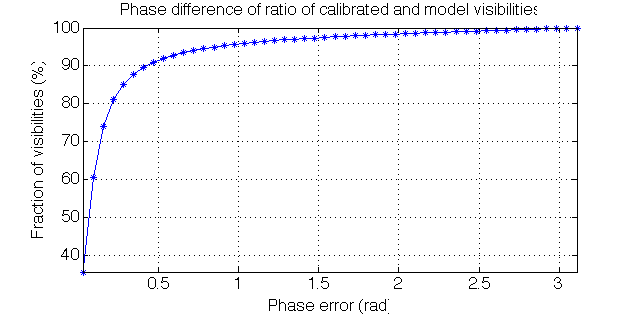
\includegraphics[width=1\columnwidth]{Figs/ph_err_54873657_cumsum}}

\caption{\label{fig:The-model-amplitude}The amplitude and phase errors of
calibrated visibilities compared to the fit model. }
\end{figure*}


Figure   \ref{fig:Major-and-minor}   shows   the   longer  term   behaviour   of
instantaneously calibrating every timeslice of  the timeseries from dataset 1 to
convergence. An average  of close to 40 iterations are taken  in the minor cycle
(spread over the 3-4 major cycle iterations) in the initial part of the dataset,
while this reduces to about 30  iterations in the latter half of the observation
with about  3 major cycles. This small  reduction in the number  of minor cycles
indicates towards the  steep convergence of StefCal, which  results in a smaller
number of  minor iterations for the later  major cycles due to  a better initial
estimate. The convergence  criteria is based on the rate  of change of estimated
parameters slowing to a predefined value, rather than a threshold on the fitting
error. The  final slopes for  the major  and minor cycle  are also shown  in the
figure.

\begin{figure*}[tbh]
\centering
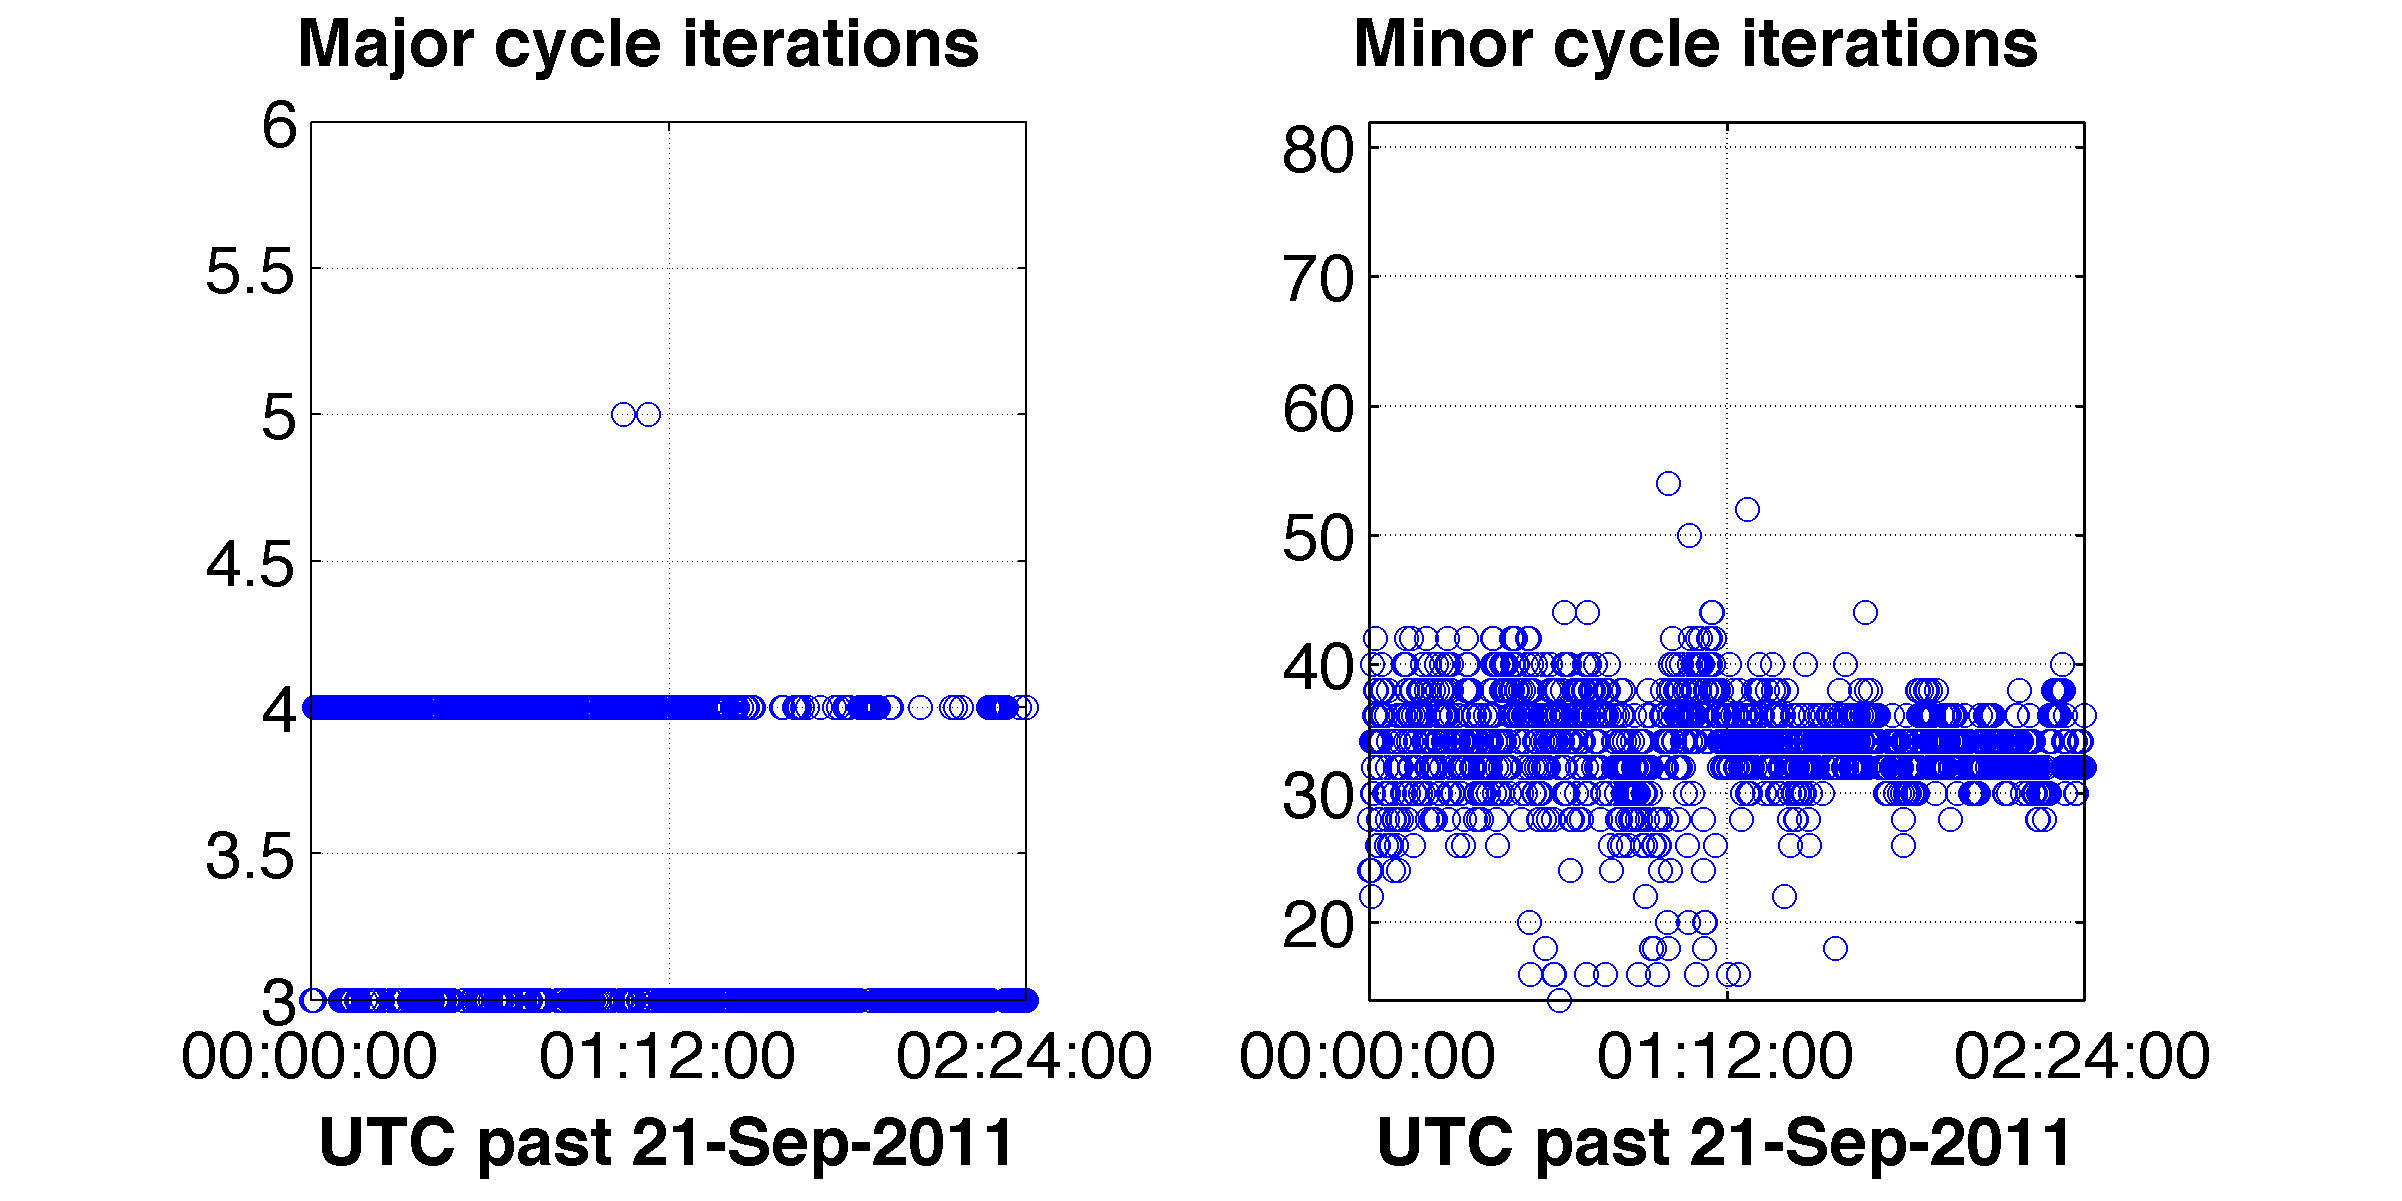
\includegraphics[width=0.7\textwidth]{Figs/SB000_ch30-35_5sec_3hr_9_convcalsol_bin_iter}

\caption{\label{fig:Major-and-minor}Number of iterations of major and minor
cycles, and their error surface slopes after convergence. The first
half of the dataset (set 1) is affected by the flaring Sun, requiring
a larger number of iterations for convergence.}
\end{figure*}


%% \textcolor{red}{<TODO:} Additional stuff: error in the estimated parameters
%% against the number of iterations on a typical snapshot?>


\subsection{Accuracy of tracking calibration}

We present the performance of our algorithm on datasets 1 and 2. The performance
is tuned for maximum computational efficiency by restricting the major and minor
cycles to  just one. The  tracking solutions are  compared to those  obtained by
calibration  to convergence.  The comparison  is carried  out on  the estimation
parameters consisting  of DIE gains, the  model source flux  estimates and their
positions. The system noise is excluded from the comparison.(Why?)

\begin{figure*}[tbh]
`\center{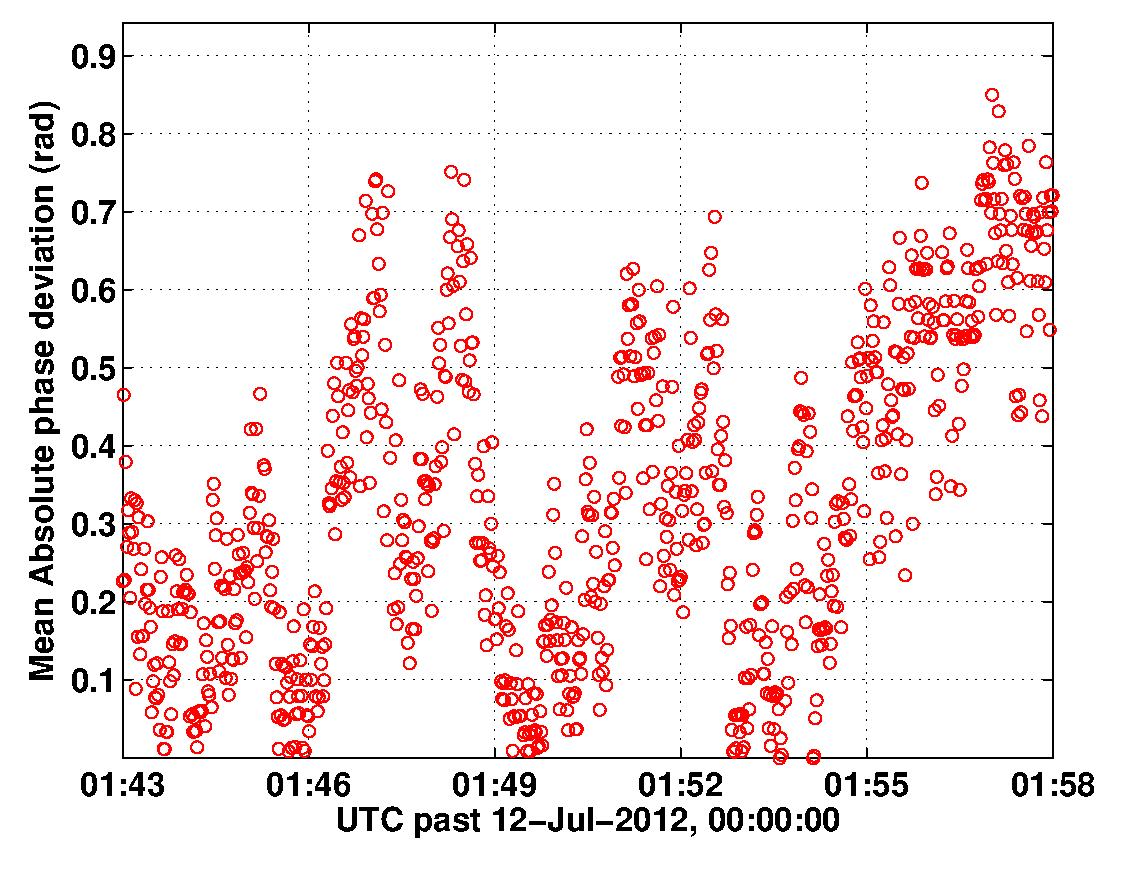
\includegraphics[width=0.7\paperwidth,height=7cm]{Figs/cmpcalsol}}\caption{\label{fig:The-error-timeseries}The error timeseries of tracking
calibration solutions as compared to those obtained after iterating
to convergence. }
\end{figure*}


Figure   \ref{fig:The-error-timeseries}   shows   the  variation   of   tracking
calibration solutions,  relative to  those obtained via  convergent calibration.
The  error  is obtained  via  a  mean square  criteria,  and  is normalized  per
parameter. The dataset is characterized  by a disturbed ionosphere, probably due
to  the recombining of  the disturbed  plasma. This  results in  short timescale
amplitude  and position  jitter of  the  model sources.   These are  effectively
tracked  by  the   short  cadence  calibration,  as  can   be  seen  in  Section
\ref{sub:iono-effect-on-calib}.  The  tracking  calibration solution  error  per
parameter rises  during certain times due  to slight variations  in model source
position estimates between the tracking and convergent calibration.


\subsubsection{Phase stability}

The collective phase  of a receiver path is more  susceptible to disruption than
the amplitude,  primarily due to the  rapid phase distortions  introduced by the
ionosphere. Such a  phase distortion also contributes more  (ref or summary?) to
the noise due to calibration artifacts than the amplitude.

Figure  TODO shows  a similar  metric, but  during a  day time  observation with
significant contribution  from the  Solar disc (dataset  1). We note  the larger
error during the initial part of the observation,


\subsubsection{Light curve stability}

An important  aspect of calibration is  the flux recovery of  sources with known
fluxes. This is  now demonstrated for our calibration scheme.   We carry out DFT
imaging of data calibrated with  the tracking calibration algorithm, and extract
out  fluxes of  some field  sources in  the observation.   This is  presented in
Figure \ref{fig:Light-curves-of}. One can see that  the dominant source of variation in the extracted
flux is  due to systematic variations  on the short scale,  most probably caused
due  to  the  ionosphere.  This  limits  the ultimate  noise  on  the  extracted
light-curve.

\begin{figure*}[tbh]
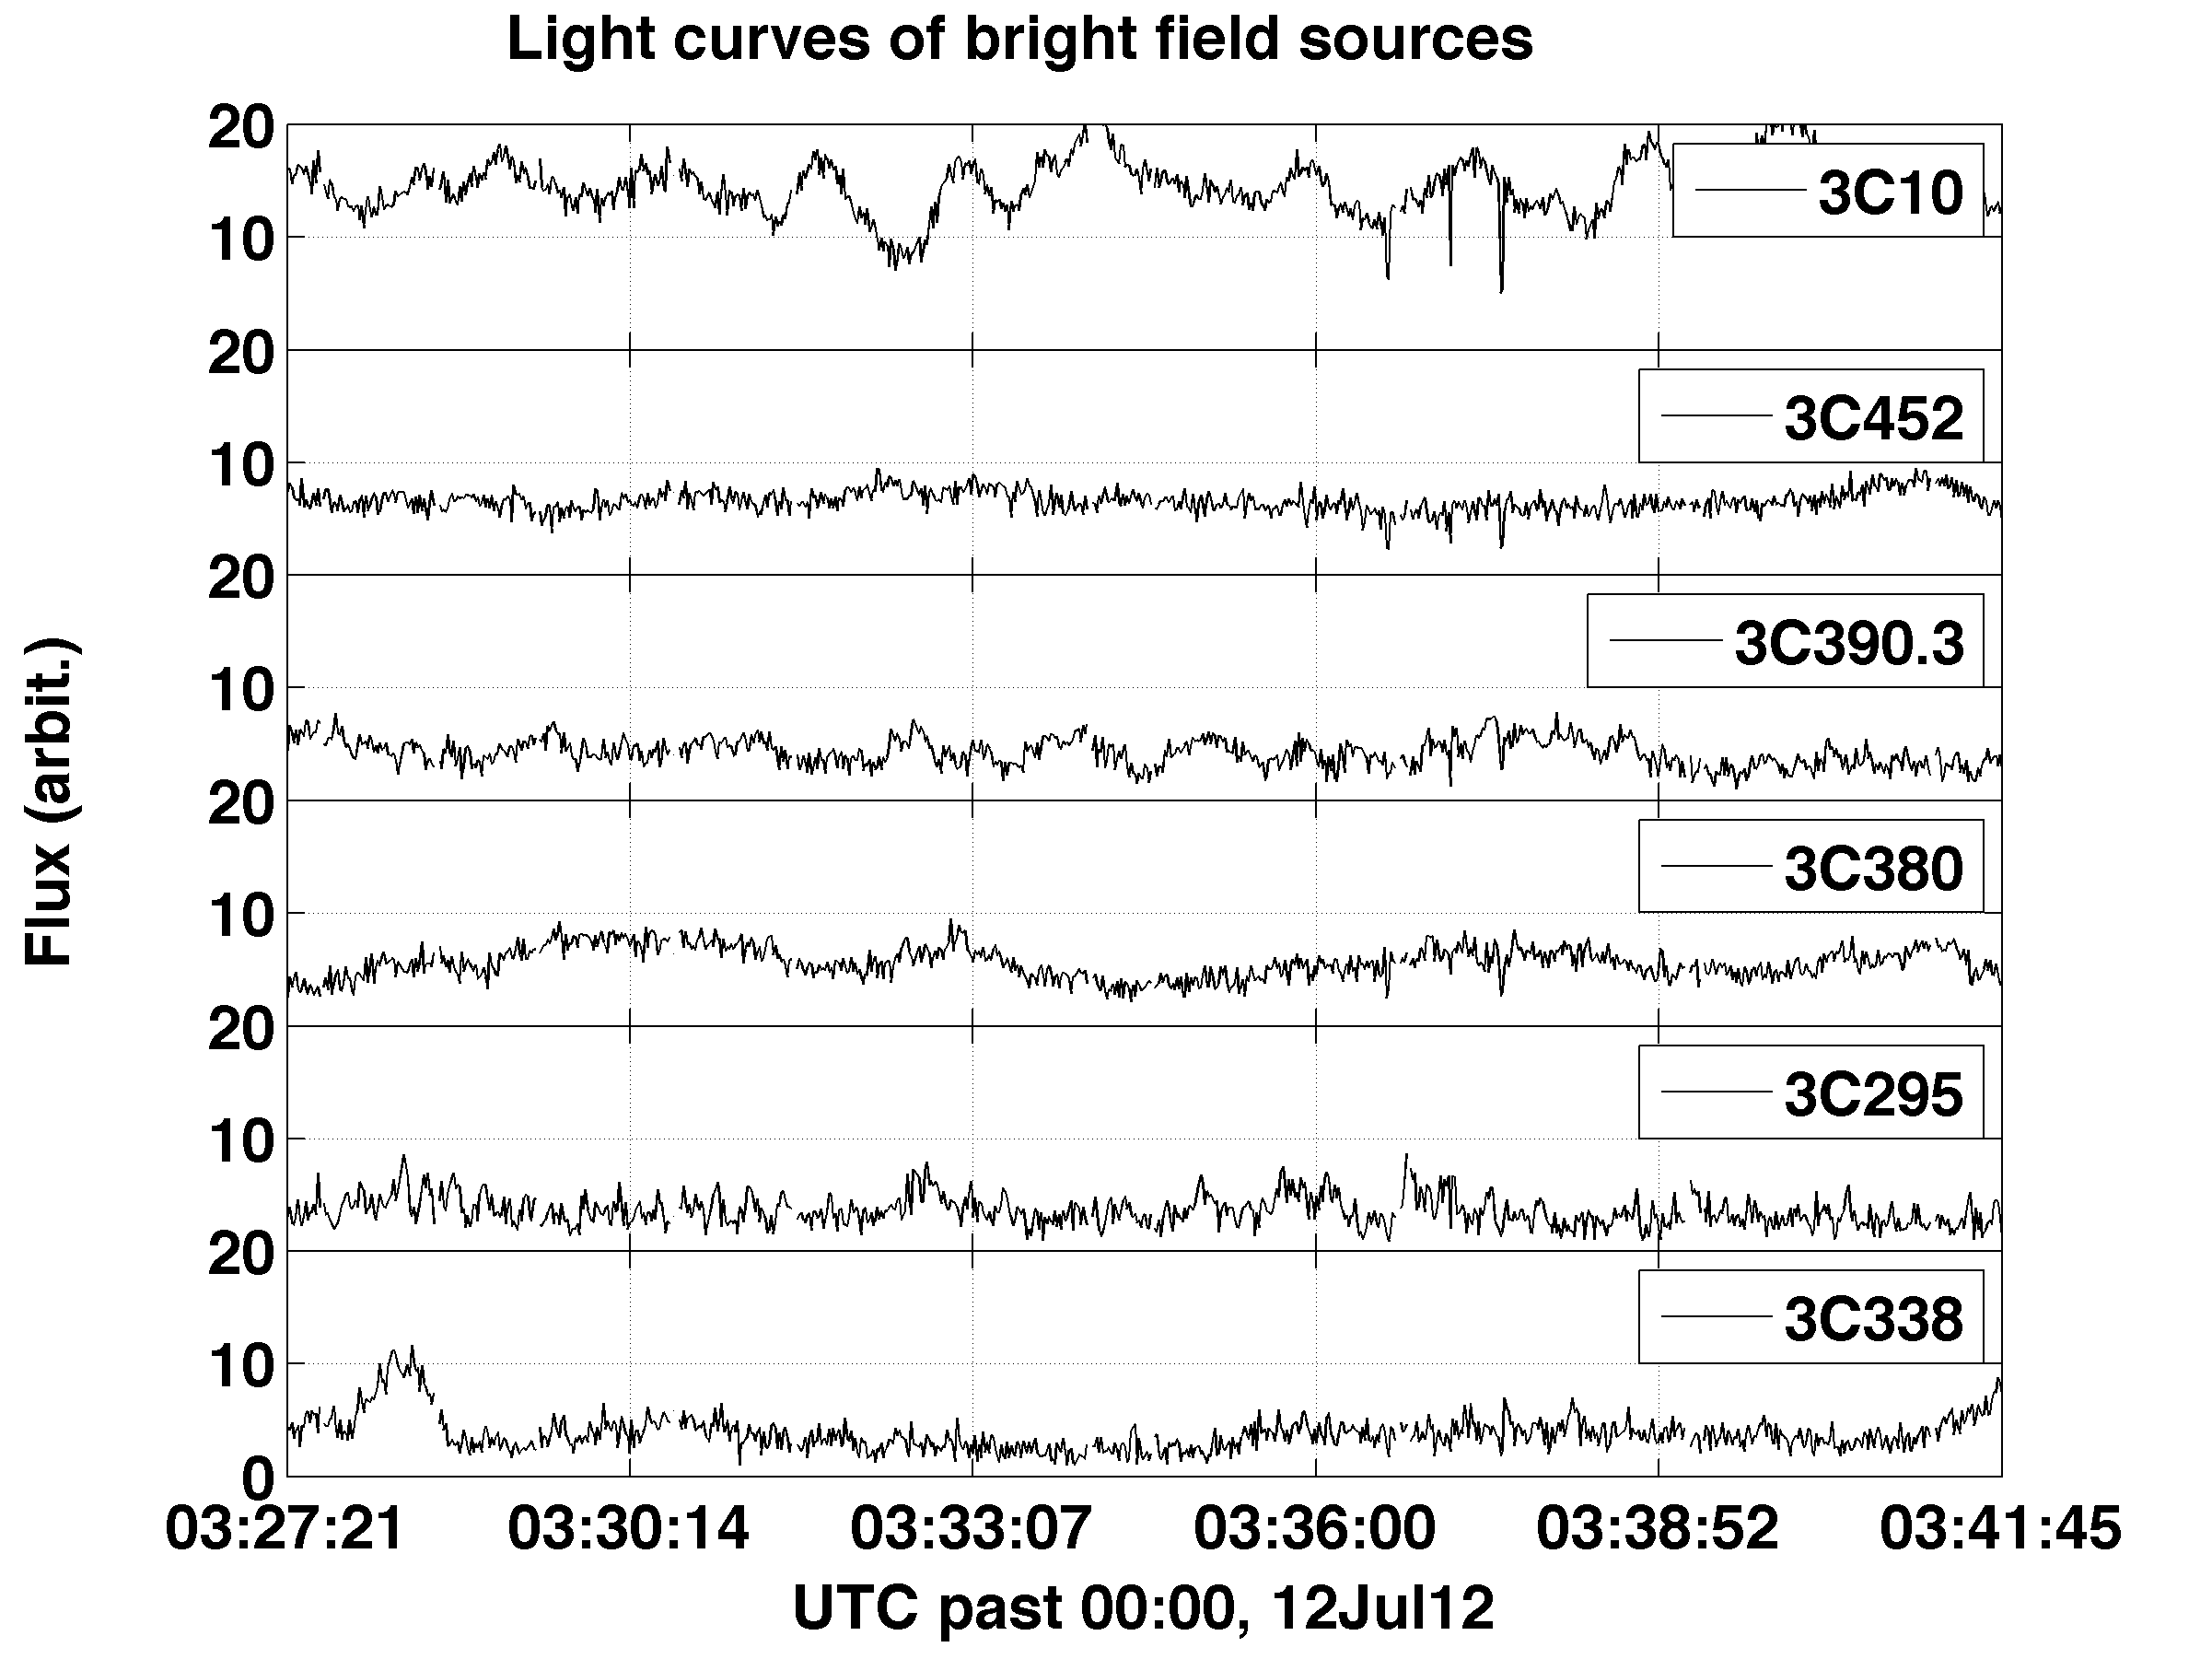
\includegraphics[width=1\textwidth]{Figs/SB002_LBA_OUTER_SPREAD_1ch_6_convcal_7_el_fftimg_bin_save_mat_tseries}

\caption{\textcolor{red}{\label{fig:Light-curves-of}}Light curves of a few
field sources from images of the calibrated visibilities.}
\end{figure*}
The position offset  of the extracted sources as  compared to cataloged position
shows  no  significant  bias,  leading  to  the conclusion  that  there  are  no
significant systematic calibration errors.


\subsection{\label{sub:iono-effect-on-calib}Effect of the ionosphere on AARTFAAC
calibration}

The AARTFAAC observes sources through the  ionosphere, which is a time and space
variable refractive  medium. Its very short  baselines result in  a strong phase
coherence across  the array, while  its rapid calibration cycles  oversample the
ionospheric phase coherency timescales. However,  its wide field of view results
in diminished  phase coherence across  the field of  view. The phase of  a radio
wave traveling  through the ionosphere can  be rotated due  to spatially variant
refractions and  propagation delays introduced by the  plasma. Thus, propagation
delay differences can  be introduced between array elements,  resulting in phase
errors in the estimated visibilities. Since the delay per antenna depends on the
Total Electron  Content (TEC) of the ionosphere  along the line of  sight to the
source, and  hence on antenna position,  a phase correction which  can vary over
the  field  of   view  needs  to  be  applied   for  calibrating  low  frequency
observations, and a single phase correction per antenna (as obtained by SelfCal)
is insufficient. Ionization  of the ionosphere during the day  by the Solar wind
and photo-ionization  is balanced by  recombination during the night.  These can
cause  bulk  variations $\left(\sim10x\right)$  in  large  scale  TEC with  slow
temporal variations,  as well as  fluctuations on relatively small  temporal and
spatial scales ($\sim0.1\%$  variations over a few Km and over  10s of secs). If
the rapid TEC fluctuation sets up an instantaneous spatial phase gradient across
the array in the direction of a source, an apparent position shift of the source
is seen.  However, if  the phase  structure function varies  from a  gradient, a
deformation of the source structure  may result due to defocussing, resulting in
a reduction of the source peak flux.

These  effects  influence the  transient  sensitivity  of  the AARTFAAC  in  two
ways. Firstly, the phase errors cause scattering of source power into sidelobes,
affecting the reliability  of the extracted lightcurves.  Secondly,  a change in
apparent  source  shape  leads  to  an  increase  in  residual  sidelobes  after
deconvolution, as the mean source model deviates from the apparent instantaneous
sky, and the source subtraction is incomplete. These residual sidelobes increase
the background noise level, and can introduce spurious structure into the image.

The very  short baselines of  the AARTFAAC array  were expected to  be minimally
affected by  the latter. Recent  results \citep{intema2009ionospheric}, however,
have indicated  towards the  presence of  a turbulent layer  below the  peak TEC
which has more power in the smaller  scale fluctuations than in the case of pure
Kolmogorov turbulence. This  is exacerbated by the very large  fields of view of
the AARTFAAC.  These are expected  to be larger  than the typical scale  size of
ionospheric fluctuations  when projected onto ionospheric  heights, resulting in
\emph{anisoplanatic }conditions  where the  ionospheric phase error  varies over
the FoV of each antenna.

Note that  short baselines between closely  spaced stations were  expected to be
immune to  ionospheric effects, and are  expected to play a  significant role in
constraining    the     calibration    of    the     full    LOFAR    instrument
\citep{vdTol2007selfcallofar}.

During our  test observations, the  most common effects  seen seem to be  due to
small 'bubbles'  of turbulent plasma, which  are able to  affect sightlines from
different  antennas.  This  results  in  high frequency  scintillations  of  the
brightest     sources,     as    well     as     position    wander.      Figure
\ref{fig:Estimated-flux-of} shows the effect  of the ionosphere on the estimated
flux of CasA, over the course of $\sim18$ mins for dataset 3.

\begin{figure*}[tbh]
\center{
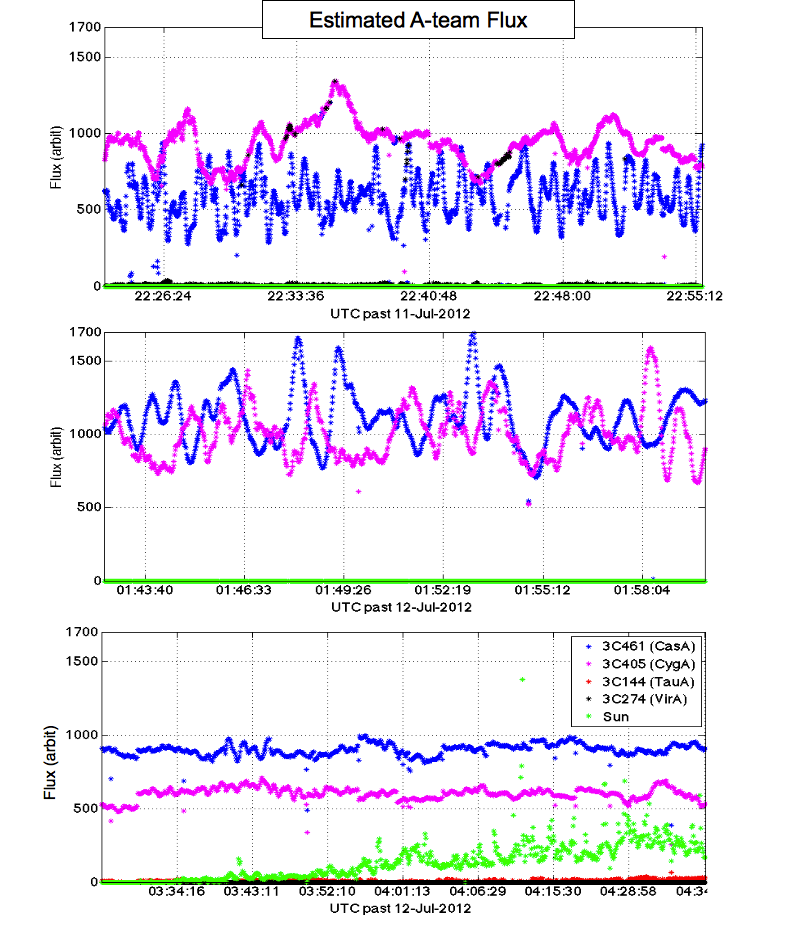
\includegraphics[width=\textwidth]{Figs/combined_plot_portrait}

\caption{\label{fig:Estimated-flux-of}Estimated flux  of model sources  CasA and
  CygA randomly sampled over \textasciitilde{}7 Hrs. The scintillations point to
  ionospheric electron  fluctuations with linear  sizes comparable to  the short
  baseline lengths of the AARTFAAC.}
}
\end{figure*}


The variation  of the position of  model sources from catalog  locations under a
typical ionosphere is  demonstrated by Figure \ref{fig:Deviation-of-the}.  Here,
the   actual   position   estimates   have   been   obtained   using   the   WSF
algorithm. Systematic  variations of upto  20\% of a  PSF are present  (are they
sufficient t cause a calibration bias?), and are seen to be a strong function of
frequency, as expected due to the ionosphere.

\begin{figure}[tbh]
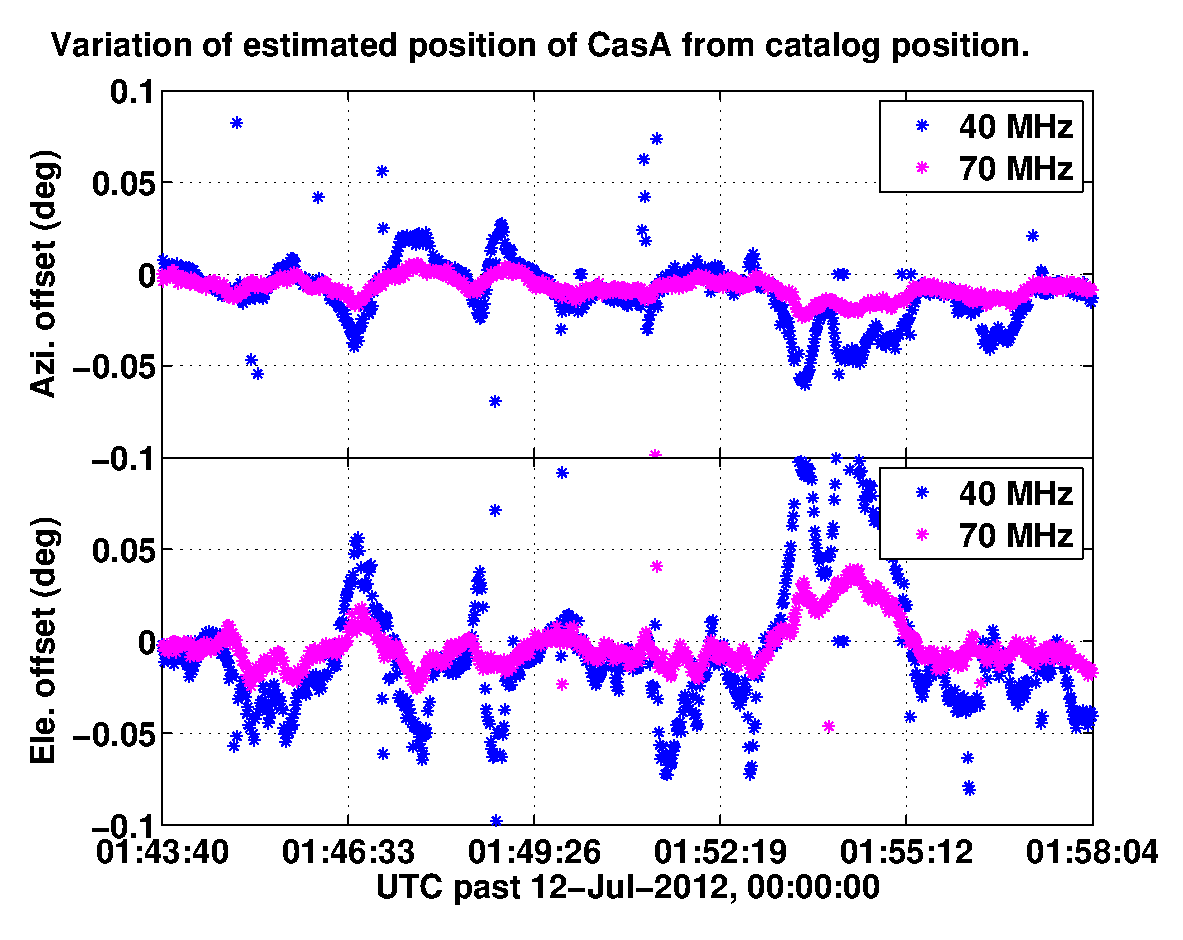
\includegraphics[width=1\columnwidth]{Figs/CasAsrcposoff}

\caption{\label{fig:Deviation-of-the}Deviation of the WSF estimated position
of 3C461 over \textasciitilde{}1000 sec, as compared to its catalog
position. Shown at two frequencies separated by \textasciitilde{}30MHz.}
\end{figure}


Tracking such  behaviour is the primary  reason for carrying  out near real-time
calibration, more so  because the streaming nature of  the application precludes
multiple  calibration   passes  through  the   recorded  visibilities.  Tracking
calibration is  able to recover such  short term affects  quite successfully, as
can be seen from the above figure.

Such a direction dependent correction  is estimated and carried out only towards
the directions of  a few model sources. Thus, the  instantaneous gains and model
source fluxes  and positions are estimated  such that the flux  and positions of
model sources  are consistent. This does  not apply to the  other sources within
the  field of  view. Hence,  we have  observed that  the light  curves  of field
sources only  a few degrees away from  the model source can  have high frequency
flux fluctuations contributed due to the ionosphere. From the test observations,
this places another  constraint on the achievable noise in  our images, which is
$\sim TODO$ Jy.

\emph{Time/spectral  bin  for  calibration:  }The basic  requirement  of  either
calibration approach is enough SNR  from the model sources, for consistency with
the specified skymodel.  At the low frequencies of  operation, the instrument is
sky-noise dominated, with the brightest model sources contributing at least ??\%
of the  received flux. The Galactic emission  is also very bright  at the lowest
frequencies, but  a spatial  filtering is  applied to reduce  its effect  on the
data.  Based on simulations{[}Wijnholds{]},  the approaches  have been  known to
require  a minimum  of  TODO dB  SNR on  the  data. Thus,  under most  observing
conditions,   a   time  bandwidth   product   (TBP)   of   at  least   TODO   is
required. Considering  our wide  field of view,  bandwidth smearing  effects can
start affecting  sources (3dB attenuation?) at  the edges of our  field after an
averaging of \textasciitilde{}TODO Hz. Thus,  in our standard autonomous mode of
operation, we choose a TBP of TODO Hz and TODO sec.


\subsection{\label{sub:Computational-performance}Computational performance}
The AARTFAAC All-sky monitor is a realtime system, requiring it to keep up with
incomming datastreams from the correlator. Furthermore it is desired that the
latency of the imaging pipeline remains below $1$s. In order to achieve these
requirements the parallelizable components need to be identified, see Figure
\ref{fig:pipeline}. Each stream represents a subband which itself holds a
number of channels. A single channel corresponds to a single ACM, or set of
visibilties that requires calibration. \\ 
As such, we can process each subband independently and each channel within a
subband independently for that subband, giving us two stages of parallellism.

\begin{figure}[tbh]
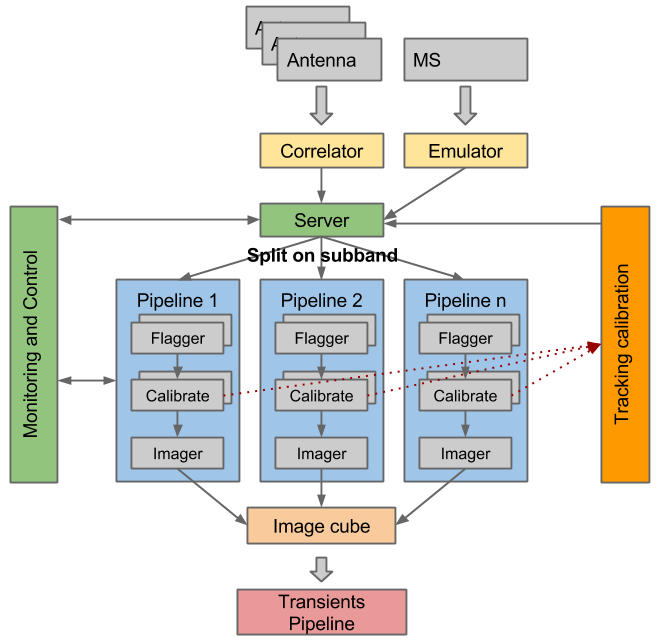
\includegraphics[width=1\columnwidth]{Figs/pipeline-design}\caption{\label{fig:pipeline}
High level overview of the imaging-pipeline design. We can see the two stages
of parallelism. The first stage splits the visibilities on each subband,
processed by a pipeline.  The second stage splits each subband into channels
which are each flagged and calibrated, depicted by the stacked rectangles.
Finally all channels within a pipline are imaged and combined into an image
cube for further analysis.}
\end{figure}

\subsubsection{Architectual dependent description}
As the calibration algorithm's major, minor cycle and the WSF are iterative in
nature, we chose a cpu based approach using C++ as the main language in
combination with Eigen3 \citep{eigenweb}. Eigen 3 is A high performance
template library for linear algebra with a clean and expressive API. \\
The high throughput pipeline is built on the Pelican (TODO REF)
framework, which is suitable for creating a loosely coupled realtime worker
pool (pipelines), fed by a single server in a first come, first served mode.
Each pipeline receives a single subband for timestep $t$ from the server, next
it flags bad antennae and calibrates each individual channel per thread and
finally creates a single image by combining the channels again, see Figure
\ref{fig:pipeline}.

\subsubsection{Performance results}
The system processes a channel per cpu core i.e. per thread, we define the
performance as the processing time of a single channel. See table
\ref{tab:Performance-results} for an overview of the time spent the various
calibration functions. Note that these timings were obtained for data that has
a calibration solution. When no solution is found, the timings depend on the
maximum number of iterations allowed in both the minor and major cycle and the
WSF algorithm. \\
The computational cost is dominated by the model source position estimation,
while an individual iteration of DIE calibration is seen to be quite
light-weight. We measured the total time (flagging, calibration, imaging) of a
subband with $N$ channels using $N$ cpus to be $250$ ms ($\sigma = 15$) for
nighttime data and $TODO$ ms ($\sigma = TODO$) for daytime data on a Intel(R)
Core(TM) i7-2600 CPU @ 3.40GHz.
\begin{table*}[tbh]
\center{%
\begin{tabular}{|c|c|c|c|c|}
\hline 
Function & Time measured & Time spent & Time measured & Time spent\tabularnewline
\hline 
\hline 
Initialization & Night & 5\%  & Day & -\tabularnewline
\hline 
Model source pos est. & Night & 83\%  & Day & -\tabularnewline
\hline 
Major cycle & Night & 7\%  & Day & -\tabularnewline
\hline 
Minor cycle & Night & 5\%  & Day & -\tabularnewline
\hline 
\end{tabular}}

\caption{\label{tab:Performance-results} Overview of the time spent in
calibration function blocks for various datasets (daytime and nighttime). We
measured the overall time (flagging, calibrating, imaging) of an ACM to be
$250$ ms ($\sigma = 15$) for nighttime data and $X$ ms ($\sigma X$) for daytime
data using current generation hardware.}
\end{table*}
\textcolor{red}{TODO: Obtain daytime results, explain difference}


%% \begin{figure}[tbh]
%% 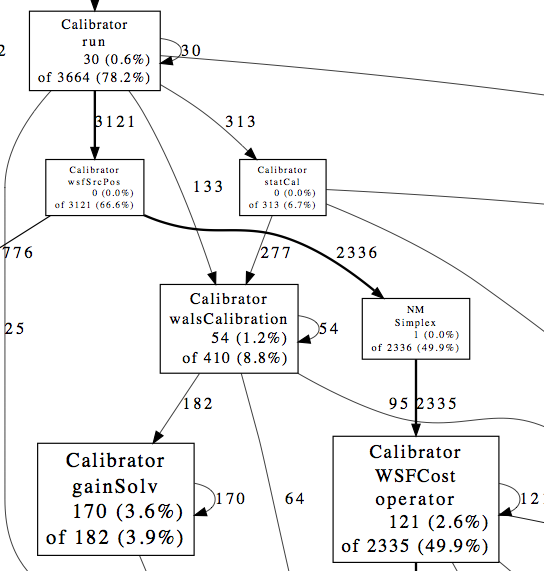
\includegraphics[width=1\columnwidth]{Figs/pipeline_profile}\caption{\label{fig:Profile-of-calibration}Profile of calibration pipeline}
%% \end{figure}



\subsection{\label{sub:Stability}Stability}

The stability of  the tracking calibration can be gauged from  the errors on the
estimated parameters. These  are most likely to be  non-convergence of the model
fitting, or  biases due  to model  fitting errors. The  former can  be due  to a
complete  model mismatch  because of  the flaring  Sun or  intense RFI,  and are
usually  easily identified  by  exploiting temporal  stability constraints.  The
latter can arise during  observations with a significantly disturbed ionosphere,
or due to low level RFI. These  are more difficult to isolate, although they can
be classified  according to  the expected behaviour  of each parameter.  To this
end, Figure  \ref{fig:gain-Temporal-stability} shows the  estimated complex gain
timeseries from a few antennas  over \textasciitilde{}7 hrs. The variance on the
estimated  phase of  the instrument  is \textasciitilde{}<TODO>  rad,  while the
amplitude has variations on the <TODO>\%.  The figure also shows the reaction of
the instrument to different observing conditions, and in conjunction with Figure
\ref{fig:Estimated-flux-of},  show a nice  segregation of  the sources  of error
into instrumental and observational.

\begin{figure*}[tbh]
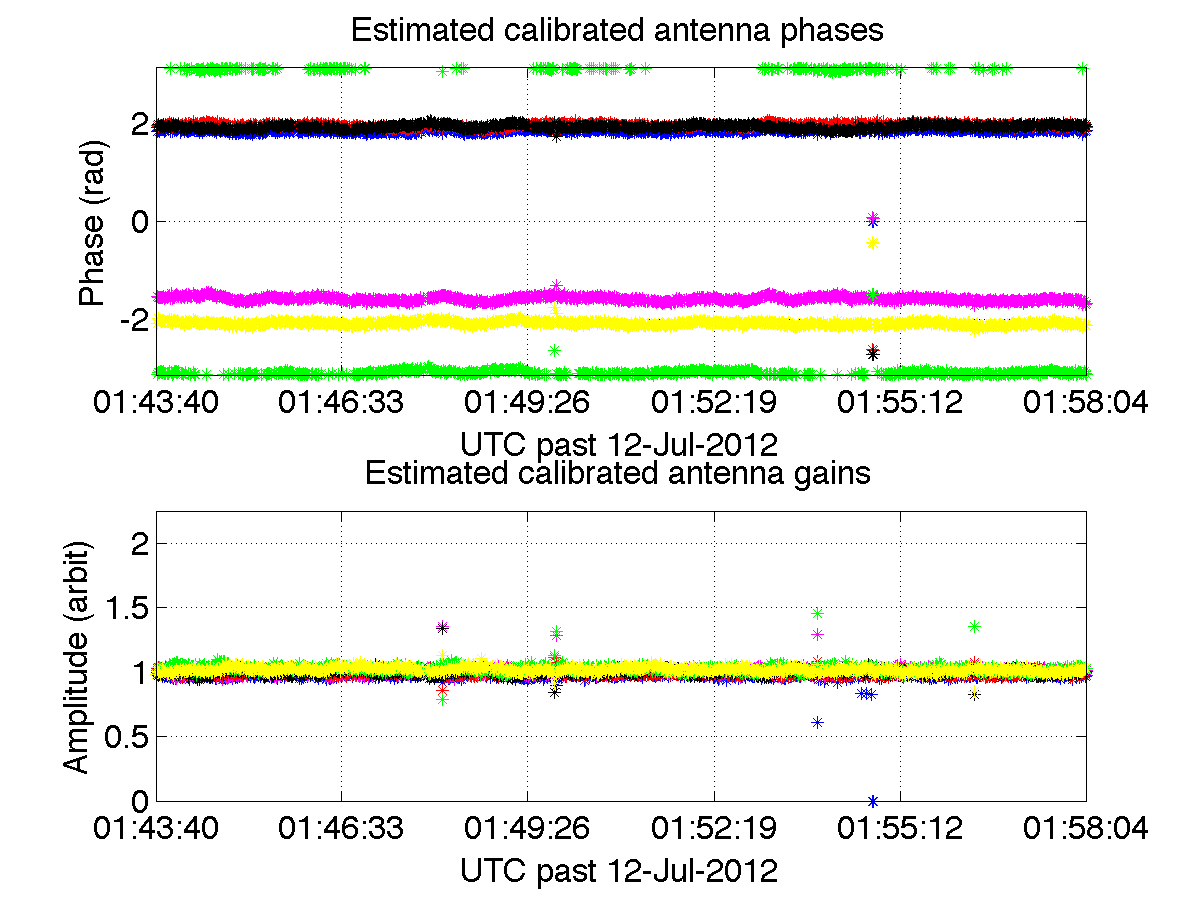
\includegraphics[width=1\textwidth]{Figs/SB002_LBA_OUTER_SPREAD_1ch_8_convcalsol_bin_gains.png}\caption{\label{fig:gain-Temporal-stability}Temporal stability of the complex
gain of a randomly chosen set of 6 antennas from the 288 AARTFAAC
antennas over a period of \textasciitilde{}7 hrs.}
\end{figure*}

\begin{itemize}
\item Comment on evening/dawn time observations, contrast with VLA 74 MHz
obs which are unusable during these times.
\end{itemize}

\subsection{\label{sub:Enhancing-the-transient}Enhancing the transient detection
sensitivity via difference imaging} The snapshot dynamic range of our calibrated
images  can  be  lower  than  expected due  to  several  reasons.  Observational
conditions like  a flaring  Sun or significant  ionospheric effects can  only be
addressed  in a limited  manner due  to latency  and computing  constraints. The
effect of spatial  filtering of diffuse emission via  visibility tapers for ease
of modeling  can give rise  to high ripples  from unmodeled flux.   Carrying out
only a  few iterations while  calibrating can lead  to partial convergence  of a
snapshot calibration. This, in turn,  can also lead to higher sidelobe confusion
noise. Further,  the ASM is expected to  hit its classical confusion  limit in a
few  10s  of seconds  of  integration,  due to  its  poor  resolution. At  short
timescales, all these effects are systematic due to the negligible change in the
sky  brightness  distribution and  instrumental  parameters,  and  hence do  not
average down on integration.

Thus, the ASM is expected to  be a confusion noise limited instrument.  Here, we
examine the temporal difference image domain as a viable alternative to snapshot
images for  transient searches, and  quantify the improvement in  sensitivity of
such images.

A  difference  image  is expected  to  have  a  higher  sensitivity due  to  the
cancellation of the abovementioned systematic effects, which should leave better
structured  Gaussian noise  in the  residual. Further,  steady sources  are also
cancelled in the  difference domain, making it an  excellent domain for searches
for short term transients. The sensitivity of the difference image can depend on
the  extent to  which systematics  cancel, which  in turn  can be  influenced by
observing conditions. The effectiveness of this domain is demonstrated in Figure
\ref{fig:Reduction-in-image}, which shows the decrease in noise with integration
time  for a  snapshot image  as well  as a  difference image,  as a  function of
integration  time.   The  theoretical   curve  shows  the   expected  $\sqrt{N}$
enhancement  on the  integration of  N timeslices,  and we  see the  noise  in a
difference image  closely following this  curve out to about  $\sim40$secs. Note
that higher  integrations are achieved  by adding consecutive  timeslices before
subtracting two images. This implies that effects like earth rotation or changes
in systematics due  to changes in instrumental parameters  over time are ignored
in    this   approach.    In   principle,    short   term    image   differences
(\textasciitilde{}secs) are enough to reduce noise amplitude by 20-30\%.

\begin{figure*}[tbh]
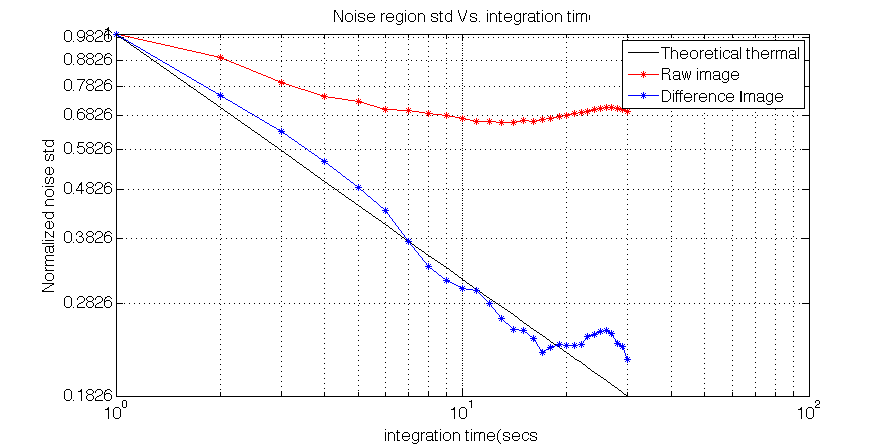
\includegraphics[width=0.9\paperwidth]{Figs/raw_vs_diff_vs_theory}

\caption{\label{fig:Reduction-in-image}Reduction in image noise as a function of
  integration  time over  raw  and differenced  consecutive  image pairs.   Each
  member of the pair being differenced is generated by averaging raw images over
  increasing  cadences.   The  difference   image  curve  closely   follows  the
  theoretically expected curve out to about a minute, after which Earth rotation
  is expected to make difference imaging ineffective.}
\end{figure*}



\section{\label{sec:Challenges-to-tracking}Challenges to tracking calibration}

The tracking calibration  scheme has been found to  be computationally effective
and is based  on the statistically efficient Stefcal.  algorithm.  There are two
categories    of   challenges    faced    by   our    approach   to    real-time
calibration. Firstly, the instantaneous calibration can become biased due to the
presence of  unmodeled signal components,  or because of  a larger error  on the
estimation  parameters on  data  with poor  SNR  due to  the  limited number  of
iterations.   These   effects   tend   to   lower  the   sensitivity   of   each
timeslice. However, the  TraP has several checks to avoid  being biased by these
inconsistencies.  Secondly,   due  to  the  feedback   in  tracking  calibration
introduced via the initial estimation, biases in the solutions can be propagated
in time.  This can lead  to unintended variations  in the extracted flux  due to
under/over estimation  of the  gain amplitudes,  and can also  lead to  a higher
deconvolution noise due to position errors on the brightest sources. This effect
is more  challenging to counter due  to the minuteness  of the bias, but  can be
countered effectively  by introducing periodic convergent  calibration cycles in
the real-time stream. We first illustrate the former set of challenges.


\subsection{Radio Frequency Interference (RFI)}

RFI mimics  a coherent source across the  array, and is usually  very bright and
sporadic, both in time and frequency. RFI can be very detrimental to a transient
machine  due  to  the  difficulty  in  its  separation  from  genuine  celestial
transients,  with  a  corresponding   increased  false  detection  rate.  Strong
terrestrial RFI  near the AARTFAAC  site has been  found to affect only  a small
fraction of  data. The high time  and spectral resolution  of calibration allows
RFI rejection to  be carried out within our pipelines  via simple sliding window
filters operating on the total received  power per ACM.  However, minor RFI does
slip  through, resulting in  a model  and data  inconsistency.  During  times of
reasonably  heavy  RFI, the  estimation  does not  converge,  and  so is  easily
distinguished.  For  tracking calibration,  the steep convergence  curve usually
generates solutions  for such timeslices which are  significantly different from
the maintained  time history, and the  timeslice is effectively  rejected by the
filters on the generated solutions.. RFI from  a single source  usually results in  the estimation
placing the brightest source in the model sky at the location of the RFI source.
This  results in  significantly different  phase  solutions, which  can also  be
trapped. This also includes effects due to lightning.

An insidious source of RFI are  reflections of terrestrial RFI (which is usually
at  low  elevations,  and  hence   trappable)  from  meteor  trails  or  passing
aircraft. These can be dim enough  to not bias the skymodel significantly, which
makes them  difficult to  filter out.  They can, however,  be trapped  by higher
level filters due to their rapid movement across the field of view.

In conclusion,  RFI is  not a  significant problem for  the AARTFAAC.   The fast
recalibration allows  us to distinguish individual RFI  corrupted timeslices and
discard  them  from further  analysis,  while weak  RFI  which  does not  affect
calibration will have to be filtered by higher layers like the TraP.

%% \textcolor{red}{<TODO>}<  Add  figure  giving  statistics of  outright  rejected
%% timeslices, and of timeslices rejected due to inconsistent models, and show that
%% this is comparable to that seen in the LOFAR paper.>

\subsection{The active Sun}

The quiet Sun  is a well-known broadband radio source at  frequencies of tens of
MHz, due to black-body radiation from  the Corona being in the Rayleigh regime .
Inspite of the radio extent of the  quiet Sun being much larger than the optical
disk, simple point  or gaussian models are adequate  for its representation with
the AARTFAAC PSF.  However, during periods of sunspot activity, small regions of
emission can extend  over several solar radii. These  typically have an inverted
spectrum, making them the brightest sources in the sky. During intense activity,
these components  can be resolved by  the AARTFAAC, thus  invalidating the point
source assumption of the Solar  model. A multi-component model which varies with
time and frequency would then be required. Presently, latency bounds prevent the
extraction of  such a model from  incoming data to update  the calibration model
dynamically  for accurate  calibration and  their effective  subtraction.  Thus,
timeslices with  a flaring Sun are  either discarded using filters  based on the
ACM total  power, or lead to  images with significantly higher  noise, which are
appropriately handled by higher level  processors. The dynamic range of AARTFAAC
images after tracking calibration is $\sim2200:1$, and so images in the presence
of the quiet Sun can be considered for transient detection.


\subsection{Creeping bias in tracking calibration}

Since both  the positions  of the  model sources as  well as  the phases  of the
antenna gains are estimated during the calibration, a biased estimate of one set
of  parameters can  be  compensated by  a corresponding change in the  other during the cost function minimization while estimating calibration parameters. This  is
especially  seen in  tracking calibration  due to  the use  of solutions  from a
previous  timeslice  as  an  initial  estimate,  which  can  be  biased  due  to
non-convergence of tracking  calibration on data with  poor SNR.  A simple solution for this has  been found to be
the periodic  recalibration to full convergence  of the incoming  data every few
minutes. This limits the bias to a small fraction of the estimates.   The effect  of this  can  be seen  on the  phases, being  subsequently
brought back on track via a convergent calibration.

%% \begin{figure*}[tbh]
%% \center{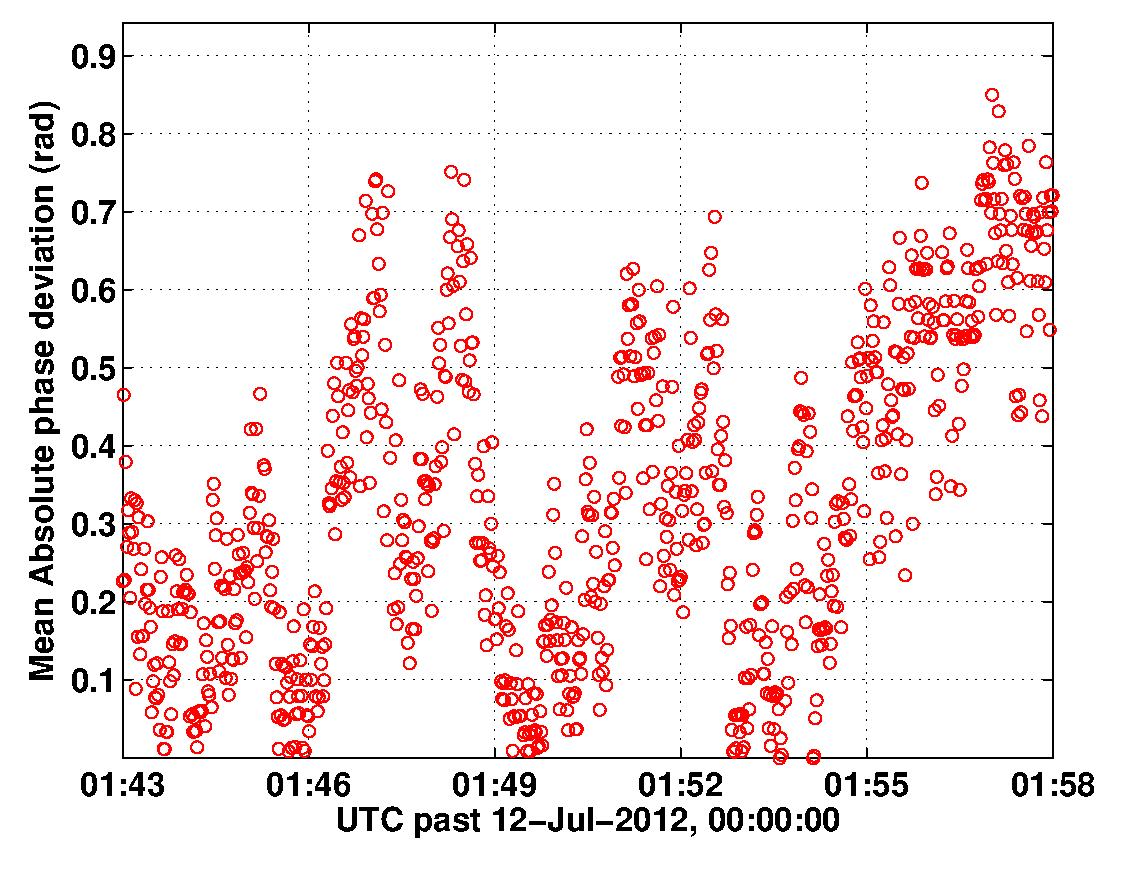
\includegraphics[width=0.7\paperwidth,height=7cm]{Figs/cmpcalsol}}\caption{\label{fig:The-error-timeseries-1}The error timeseries of tracking
%% calibration solutions as compared to those obtained after iterating
%% to convergence. }
%% \end{figure*}


%% \section{\label{sec:Discussion}Discussion}

%% The  tracking multisource  calibration  has been  found  to function  adequately
%% within  the compute  and  latency  constraints of  then  AARTFAAC ASM.  However,
%% several other factors can influence its efficiency. These are discussed below.


%% \subsection{\label{sub:Confusion,-peeling-and}Confusion, peeling and the depth
%% of deconvolution }

%% The current  algorithm determines model parameters for  the brightest unresolved
%% sources in  the sky to carry  out their effective  deconvolution.  These sources
%% account  for  almost  TODO fraction  of  the  received  power, and  hence  their
%% deconvolution  increases the  image dynamic  range to  about TODO.  However, the
%% effective noise in the generated instantaneous images is $\sim20$ Jy, accounting
%% for  the contribution  by  the  ionosphere.  Thus,  the  limitation on  achieved
%% dynamic range is constrained by  the ionospheric errors, rather than by sidelobe
%% confusion of  lower level  bright sources. Further,  does the estimation  of the
%% model source fluxes  get biased due to confusion from  background sources in the
%% relatively broad  PSF of  the AARTFAAC? What  about the simultaneous  peeling we
%% carry  out,  instead  of  peeling  individual sources  in  decreasing  order  of
%% flux?\textcolor{red}{{} <TODO> }


%% \subsection{Effect of the presence of bright transients on model based calibration}

%% The model  based Selfcal. can  be argued  to have a  high dependency on  the sky
%% model in  order to estimate the  calibration parameters. A  bright enough source
%% not present  in the skymodel  could potentially lead  to convergence to  a local
%% minimum, resulting in degraded sensitivity.  However, the relative brightness of
%% such a source needs to be substantial to affect the calibration. We carry out an
%% empirical test  for the  flux limits  which affect calibration  to the  level of
%% masking a bright transient source. However, the brightest model sources dominate
%% the  visibility amplitudes  by far,  thus  usually only  RFI can  cause a  model
%% error. \textcolor{red}{<TODO?>}
;

\section{Conclusions}

The transient  detection figure of merit of  an instrument is a  function of its
field of  view, sensitivity,  and transient detector  response time.  The latter
depends  on  a   calibration  scheme  with  the  ability   to  accurately  track
instrumental  and observing  parameters in  order to  measure source  fluxes and
positions with minimum error.

In this  paper, we have  described a real-time, wide-field  calibration strategy
optimized  for the  detection  of  bright, short-term  radio  transients at  low
frequencies, as  applicable to  the AARTFAAC All-Sky  monitor.  Our  approach is
based  on  a  model  based,  multisource self-calibration  algorithm  with  high
calibration efficiency. The fundamental challenge is to carry out the estimation
of  a  large  number  of  parameters (both  direction  dependent  and  direction
independent), within a strict latency  and compute budget. Our main contribution
in this  paper is a  calibration strategy with  a bounded latency which  we find
optimal   from    the   computation   and    image-plane   transient   detection
perspective.  Ours is a  'tracking' calibration  scheme, which  employs temporal
propagation  of parameter estimates  with a  fixed number  of iterations  of the
iterative  least  squares  solver.  We  utilize  the  expected  relatively  slow
variations of the instrumental and  observing parameters to implement a tracking
calibration  with limited iterations  (and thus  bounded latency),  and solution
propagation from previous times. We have modified the calibration estimator with
a weighting scheme  matched to the spatial Galactic  filtering required, as well
as a Selfcal  constraint appropriate for a rapidly  scintillating model sky with
image wander, caused by a  diffractive ionosphere. We show via test observations
that such  an approach is entirely feasible  for the AARTFAAC, adding  at most a
TODO\% error relative to fully convergent solutions under a variety of observing
conditions. The AARTFAAC  tracking calibration is optimized for  the precise 2-D
nature of the  ASM, its snapshot imaging mode of  operation, and its sensitivity
and field of view. Various other algorithms address a completely different class
of problems, and apply poorly to the simplified constraints of the ASM.

We  have shown  under a  variety  of conditions  that both  RFI and  ionospheric
visibility distortions do not significantly affect AARTFAAC's sensitivity, which
is  limited by  the  classical confusion  noise  caused by  its relatively  poor
resolution.  We  have further  shown that  such a confusion  noise limit  can be
effectively  breached via  difference  imaging over  short  timescales. We  have
quantified  the  efficiency  of   the  difference  image  domain  for  effective
cancellation  of   artifacts  introduced  by  the   tracking  calibration.   The
sensitivity of the  difference image is shown to  follow the expected $\sqrt{N}$
relationship  for   Gaussian  noise,  and  approaches  the   thermal  limit  for
integrations upto 10s of seconds.

Another  aspect  of  the  problem  is to  operate  autonomously  in  challenging
observing conditions  due to RFI, an  active Sun and  ionospheric effects, while
being able to filter inconsistent data from entering the tracking loop. This has
been done  by careful selection of  thresholds on relative  error of calibration
solutions,  and  coupled  with a  'coasting'  strategy,  has  been found  to  be
effective in  a real-time, autonomous  loop. With a current  C++ implementation,
the tracking  calibration operates within $\sim$  0.25 seconds on  a single time
and frequency timeslice, which is well within the compute budget.

Thus, the  tracking calibration  is an appropriate  strategy for  an autonomous,
real-time instrument like the AARTFAAC all-sky monitor.


\begin {acknowledgements}

This work  was funded by  the ERC grant  <num> awarded to Prof.  Ralph Wijers, Universitiet Van Amsterdam. We
thank the LOFAR team for building an extremely configurable instrument, allowing
the collection of  dipole level raw data for  commissioning observations for the
AARTFAAC. We thank  The Netherlands Foundation for Radio  Astronomy (ASTRON) for
support  provided in carrying  out the  commissioning observations.  Finally, we
thank  the anonymous  referee  for  helpful comments  which  have increased  the
clarity of this paper.
\end{acknowledgements}
\bibliographystyle{aa}
\bibliography{ref}

\end{document}
